\documentclass[sigconf,nonacm]{acmart}

%%
%% \BibTeX command to typeset BibTeX logo in the docs
\AtBeginDocument{%
  \providecommand\BibTeX{{%
    \normalfont B\kern-0.5em{\scshape i\kern-0.25em b}\kern-0.8em\TeX}}}

%% Rights management information. 
%% For review purposes, this block is standard.
\setcopyright{acmlicensed}
\copyrightyear{2026}
\acmYear{2026}
\acmDOI{XXXXXXX.XXXXXXX}

%% These commands are for a PROCEEDINGS abstract or paper.
% \acmConference[KDD '26]{Proceedings of the 32st ACM SIGKDD Conference on Knowledge Discovery and Data Mining}{August 3--7, 2025}{Long Beach, CA, USA}
% \acmPrice{15.00}
% \acmISBN{978-1-4503-XXXX-X/25/08}

\usepackage{mathtools}
\usepackage{amsthm}
\usepackage{bm}
\usepackage{subcaption}
\usepackage{multirow}
\usepackage{cleveref}
\usepackage{algorithm}
\usepackage{algorithmic}
\usepackage{tabularx}
\usepackage{nicefrac}
\usepackage{microtype}
\usepackage{hyperref}

% ,  Custom Macros , 
\newcommand{\TSP}{\textsc{TSP}}
\newcommand{\CVRP}{\textsc{CVRP}}
\newcommand{\ACO}{\textsc{ACO}}
\newcommand{\DyNACO}{\textsc{DyNACO}}
\newcommand{\MMAS}{\textsc{MMAS}}
\newcommand{\VRP}{\textsc{VRP}}

\newcolumntype{Y}{>{\centering\arraybackslash}X}

\begin{document}

\title[Supplementary Material]{Supplementary Material for\\Beyond Static Priors: Dynamic Neural Guidance for Large-Scale Ant Colony Optimization}

\author{Dat Thanh Tran}
\affiliation{%
  \institution{Center for AI Research, VinUniversity}
  \city{Hanoi}
  \country{Vietnam}
}
\email{dat.tt3@vinuni.edu.vn}

\author{Van Khu Vu}
\affiliation{%
  \institution{College of Engineering and Computer Science, VinUniversity}
  \city{Hanoi}
  \country{Vietnam}
}
\email{khu.vv@vinuni.edu.vn}

\author{Yining Ma}
\affiliation{%
  \institution{Laboratory for Information and Decision Systems, Massachusetts Institute of Technology}
  \city{Cambridge, MA}
  \country{USA}
}
\email{yiningma@mit.edu}

\settopmatter{printacmref=false}
\maketitle

\appendix

% Reset counters for Appendix
\setcounter{table}{0}
\renewcommand{\thetable}{A\arabic{table}}
\setcounter{figure}{0}
\renewcommand{\thefigure}{A\arabic{figure}}
\setcounter{algorithm}{0}
\renewcommand{\thealgorithm}{A\arabic{algorithm}}

% ======================================================================
% Appendix A: Methodological Details
% ======================================================================
\section{Methodological Details}
\label{app:method}

% ----------------------------------------------------------------------
\subsection{State-Aware Representation: Feature Definitions}
\label{app:state-features}

The state-aware representation (the first mechanism of dynamic neural guidance) keeps the static node features from DeepACO~\cite{deepaco} for both TSP and CVRP, and attaches additional features to candidate edges $(i,j)$ in the $K$-NN graph at every outer step $h$.
Feature~1 is the static edge distance feature used by the sparse graph; Features~2--3 capture search dynamics from the pheromone field; Features~4--6 encode the incumbent topology.

\textbf{Feature 1: Normalized Distance.}
\begin{equation}
f_1(i,j) = \frac{d_{ij}}{\bar{d}_i}, \quad \bar{d}_i = \frac{1}{K} \sum_{j' \in \mathcal{N}_K(i)} d_{ij'}.
\end{equation}
Scale-invariant by construction; ensures robustness to instance scaling.

\textbf{Feature 2: Pheromone Dispersion (Coefficient of Variation).}
\begin{equation}
f_2(i,j) = \frac{\sigma_{\tau_i}}{\bar{\tau}_i} = \frac{\sqrt{\frac{1}{K}\sum_{j'} (\tau_{ij'} - \bar{\tau}_i)^2}}{\bar{\tau}_i}, \quad \bar{\tau}_i = \frac{1}{K}\sum_{j'} \tau_{ij'}.
\end{equation}
This source-node aggregate is attached to all outgoing candidate edges from $i$ and measures local pheromone convergence: high CV indicates concentrated pheromone on few edges; low CV indicates near-uniform distribution.
Clamped to $[0, 10]$ for numerical stability.

\textbf{Feature 3: Relative Log-Pheromone.}
\begin{equation}
f_3(i,j) = \log\!\left(\frac{\tau_{ij}}{\bar{\tau}_i}\right), \quad \text{clamped to } [-5, 5].
\end{equation}
This \emph{edge-level} feature captures whether $(i,j)$ has above- or below-average pheromone relative to node $i$'s other candidates.
The log transform provides sensitivity across the full dynamic range.

\textbf{Features 4--5: Incumbent Adjacency Indicators.}
Let $b = (v_0, v_1, \ldots, v_{n-1})$ denote the current incumbent tour, with $\mathrm{succ}_b(i)$ and $\mathrm{pred}_b(i)$ denoting successor and predecessor:
\begin{align}
f_4(i,j) &= \mathbf{1}[j = \mathrm{succ}_b(i)], \\
f_5(i,j) &= \mathbf{1}[j = \mathrm{pred}_b(i)].
\end{align}
These binary features encode which edges are in the current best solution, enabling the policy to distinguish between reinforcing and perturbing the incumbent.

\textbf{Feature 6: New-Edge Indicator.}
Let $\mathrm{pos}_b(v)$ denote the position of node $v$ in the incumbent.
\begin{equation}
f_6(i,j) = \mathbf{1}\!\left[|\mathrm{pos}_b(i) - \mathrm{pos}_b(j)| \notin \{1, n{-}1\}\right].
\end{equation}
Flags edges that would introduce new structure if selected, complementing Features 4--5.

\textbf{Implementation.}
DeepACO-style static node features are computed per problem, including demand/capacity information for CVRP. The DyNACO-specific dynamic edge features are computed on GPU via PyTorch tensor operations.
Pheromone features (2--3) use stabilized bounds ($\tau_{\min}=1/K$, $\tau_{\max}=1$), ensuring $\bar{\tau}_i > 0$.
Incumbent features (4--6) are recomputed at each outer step as $b^{(h)}$ evolves.
Total dimensionality: 6 per edge, $O(n \cdot K)$ values, linear in $n$ for fixed $K$.



% ----------------------------------------------------------------------
\subsection{PPO Replay and Memory Efficiency}
\label{app:ppo-replay}

PPO replay in \DyNACO{} requires storing only lightweight summaries, not the full GNN computation graph, making importance-ratio computation tractable at 100K+ nodes.

\textbf{Stored Quantities per Outer Step.}
The incumbent successor array $\mathrm{succ}_{b^{(h)}}$ (an $n$-element integer vector) suffices to reconstruct incumbent-derived edge features (Features~4--6 in \Cref{app:state-features}) during replay, since the policy logits $z_\theta(\mathcal{S}_h)$ depend on these features.

\textbf{Stored Quantities per Inner Iteration.}
For each inner iteration $s$ within outer step $h$:
\begin{enumerate}
\item \emph{Pheromone snapshot} $\tau^{(h,s)} \in \mathbb{R}^{n \times K}$: the pheromone field at the start of iteration $s$.
\item \emph{Action trace per ant}: for each stochastic decision step $t$ of ant $a$:
  $u_t$ (current node), $j_t$ (chosen neighbor index), $\mathcal{M}_t$ (64-bit bitmask encoding feasible candidates), and a stochastic flag.
  Deterministic steps (single feasible candidate) contribute $\log p = 0$ and need not be replayed.
\item \emph{Post-refinement costs} $C(\hat{\pi}_{a,s})$ for advantage computation.
\end{enumerate}

\textbf{Sufficiency.}
The log-probability of an ant's trajectory depends only on the transition kernel and the feasible set at each step, not on the incumbent directly.
The feasible-set bitmask $\mathcal{M}_t$ is stored directly, so the incumbent is needed only for recomputing the policy's \emph{input features}, not for masking.
This allows re-computing log-probabilities $\pi_\theta(a \mid s)$ for importance sampling without storing the full GNN computation graph, keeping memory footprint low.

\textbf{Replay Procedure.}
During PPO updates, we recompute log-probabilities under the current policy $\pi_\theta$:
\begin{equation}
\bar{\ell}_a = \frac{1}{T_a}\sum_{t:\, \text{stochastic}} \!\left[ \log w_{u_t, j_t} - \log \!\sum_{j':\, \mathcal{M}_t[j']=1} w_{u_t, j'} \right],
\end{equation}
where $T_a$ is the number of stochastic steps, $w_{u,j} = \tau_{u,j}^\alpha \cdot \eta_{u,j}^\beta \cdot \exp(z_\theta(u,j))$, and the denominator is restricted to feasible candidates via the stored bitmask.
Per-decision normalization by $T_a$ ensures importance ratios $r_{a,s} = \exp(\bar{\ell}_a^{\text{new}} - \bar{\ell}_a^{\text{old}})$ are comparable across ants with varying numbers of stochastic decisions.

\textbf{Memory Footprint.}
Peak GPU memory remains near-linear in $n$ because all learned inputs live on the sparse $K$-NN graph rather than a dense $n \times n$ matrix.
In the full implementation, \DyNACO{} uses 0.35\,GB at TSP-10K and 3.11\,GB at TSP-100K, while dense constructive and neural-ACO baselines run out of memory at larger scales (Appendix~\ref{app:hardware}).


% ======================================================================
% Appendix B: Environment and Backend
% ======================================================================
\section{Environment and Backend}
\label{app:backend}

This section provides a detailed description of the perturbation-based ACO environment described in the main paper, covering the ant construction procedure, scope-restricted refinement, and CVRP-specific capacity handling.

% ----------------------------------------------------------------------
\subsection{Perturbation Algorithm}
\label{app:perturbation}

Following~\cite{faco}, ants perform $M$ relocation steps starting from the incumbent $b$, where node selection follows the neurally-shaped kernel $p^\theta$.
Algorithm~\ref{alg:perturbation-app} provides the full procedure.
Each ant touches at most $O(M \cdot K)$ edges, where $M \ll N$ and $K{=}32$, independent of problem size.

\begin{algorithm}[h]
\caption{Perturbation-Based Ant Construction}
\label{alg:perturbation-app}
\begin{algorithmic}[1]
\STATE \emph{Input:} Incumbent tour $b$, starting node $u_0$, max new-edge steps $M$, shaped kernel $p^\theta$
\STATE $\text{tour} \leftarrow \text{copy}(b)$; $\text{visited}[u_0] \leftarrow \text{true}$; $\text{new\_edges} \leftarrow 0$
\STATE $\text{checklist} \leftarrow \{u_0\}$; $u \leftarrow u_0$; $\log p \leftarrow 0$
\WHILE{$\text{new\_edges} < M$ \AND not all nodes visited}
    \STATE $\mathcal{C} \leftarrow \{v \in \mathcal{N}_K(u) : \neg\text{visited}[v]\}$ \COMMENT{feasible candidates}
    \IF{$|\mathcal{C}| = 0$}
        \STATE $v \leftarrow$ fallback to backup list or greedy
    \ELSIF{$|\mathcal{C}| = 1$}
        \STATE $v \leftarrow$ the single candidate \COMMENT{deterministic, $\log p$ unchanged}
    \ELSE
        \STATE Sample $v \sim p^\theta(\cdot \mid u)$ restricted to $\mathcal{C}$
        \STATE $\log p \leftarrow \log p + \log p^\theta(v \mid u)$
    \ENDIF
    \IF{$(u, v) \notin \text{edges}(b)$} \COMMENT{not adjacent in \emph{incumbent}}
        \STATE $\text{new\_edges} \leftarrow \text{new\_edges} + 1$
        \STATE $\text{checklist} \leftarrow \text{checklist} \cup \{u, v, \text{pred}(v)\}$
    \ENDIF
    \STATE \textsc{Relocate}(tour, $u$, $v$) \COMMENT{move $v$ to successor of $u$; $\le 3$ edge changes}
    \STATE $\text{visited}[v] \leftarrow \text{true}$; $u \leftarrow v$
\ENDWHILE
\STATE \emph{Return:} tour, checklist, $\log p$
\end{algorithmic}
\end{algorithm}

% ----------------------------------------------------------------------
\subsection{Scope-Restricted Refinement (SRR)}
\label{app:credit}

\subsubsection{The Flaw of Truncated Refinement}
Standard neural-guided approaches face a fundamental trade-off: unrestricted local search (LS) erases the policy-gradient credit signal (gradient washout), whereas restricted LS yields suboptimal solutions.
DeepACO~\cite{deepaco} employs truncated refinement, limiting 2-opt to a fixed budget (e.g., $N/4$ swaps).
While this preserves partial dependence on the neural construction, it leaves tours in a semi-converged state.
To compensate, DeepACO applies Neural Local Search (NLS), injecting neural priors into the swap operator, which requires repeated neural inference ($10{\times}$) per solution and becomes intractable for $N > 10{,}000$.

\subsubsection{The ``BFS Repair'' Mechanism}
\DyNACO{} exploits the structure of perturbation-based search.
Let $\mathcal{B}^*$ be an incumbent that is 2-opt optimal.
The policy generates a perturbation, replacing edges $E_{\text{rem}} \subset \mathcal{B}^*$ with $E_{\text{add}}$, yielding $\mathcal{B}'$.
Since $\mathcal{B}'$ is suboptimal only in the topological vicinity of $E_{\text{add}}$, SRR initializes a checklist with the endpoints of $E_{\text{add}}$ and propagates improvements outward in a breadth-first manner, bounded by the extent of the perturbation-induced displacement.

\textbf{Optimality.}
If SRR terminates with an empty checklist, the resulting tour $\mathcal{B}''$ is 2-opt optimal under the candidate-graph move set.

\begin{proof}
Let $\mathcal{C} \subseteq E(\mathcal{B}'')$ denote the set of edges created or modified during the perturbation and subsequent repair, and let $\bar{\mathcal{C}} = E(\mathcal{B}'') \setminus \mathcal{C}$ denote the remaining edges.
By construction, every edge in $\bar{\mathcal{C}}$ is identical to its counterpart in $\mathcal{B}^*$.
Consider an arbitrary 2-opt move involving edge pair $(e_1, e_2)$ in $\mathcal{B}''$.
There are three cases:
\begin{enumerate}
    \item \emph{Both $e_1, e_2 \in \bar{\mathcal{C}}$}: These edges and their neighborhoods are unchanged from $\mathcal{B}^*$. Since $\mathcal{B}^*$ is 2-opt optimal, no improving swap exists.
    \item \emph{At least one of $e_1, e_2 \in \mathcal{C}$}: SRR initializes its checklist with the endpoints of all edges in $E_{\text{add}}$ and propagates to any node whose incident edges are modified during repair. An empty checklist at termination certifies that no candidate-graph 2-opt move involving any edge in $\mathcal{C}$ is improving.
    \item \emph{Cross-boundary}: If $e_1 \in \mathcal{C}$ and $e_2 \in \bar{\mathcal{C}}$, case~2 already covers $e_1$'s endpoint, and the BFS propagation would have reached $e_2$ if an improving swap existed.
\end{enumerate}
Since all cases are exhausted, $\mathcal{B}''$ admits no improving 2-opt move under the candidate-graph move set.
\end{proof}

\textbf{Comparison with DeepACO.}
DeepACO truncates search and compensates with NLS.
SRR runs to convergence within its scope, achieving 2-opt optimality under the candidate-graph move set while preserving the policy-reward causal link without neural overhead during LS.

% ----------------------------------------------------------------------
\subsection{CVRP Backend Details}
\label{app:cvrp}

For CVRP, the policy follows the DeepACO feature convention for static node inputs, including demand/capacity features. DyNACO adds the same dynamic edge-state features as in TSP, derived from pheromone and incumbent information. CVRP-specific feasibility logic is handled by the backend, which masks infeasible transitions and restricts local-search moves to capacity-preserving operations.

\subsubsection{Capacity-Aware Relocation}
We maintain an explicit multi-route structure using linked lists, where each route $r$ tracks its current load $L_r$.
Transitions to node $j$ are masked if $\text{Load} + d_j > Q$ (capacity exceeded).
Specifically:
\begin{enumerate}
    \item \textbf{Same-route} ($r_u = r_v$): Always feasible; reordering within a route preserves load.
    \item \textbf{Cross-route} ($r_u \neq r_v$): Feasible only if $L_{r_u} + d_v \leq Q$.
    \item \textbf{Depot target} ($v = 0$): Triggers a route split; always feasible.
\end{enumerate}
The new-edge counter tracks cross-route edges specifically, ensuring sufficient inter-route perturbation for effective local search.

\subsubsection{Scope-Restricted CVRP Local Search}
The LS phase applies four operators restricted to the checklist of perturbed nodes:

\textbf{Intra-Route 2-opt.}
For each checklist node $u$, we examine 2-opt moves within $u$'s route, scanning $K$-nearest same-route neighbors.

\textbf{Inter-Route Relocate.}
For cross-route pairs $(u, v)$ with $u$ in the checklist, we evaluate relocating $u$ adjacent to $v$, subject to $L_{r_v} + d_u \leq Q$.

\textbf{Inter-Route Swap.}
We evaluate swapping positions of $u$ and $v$ between routes, requiring $L_{r_u} - d_u + d_v \leq Q$ and $L_{r_v} - d_v + d_u \leq Q$.

\textbf{2-opt* (Cross-Route Segment Exchange).}
We evaluate exchanging route tails, checking cumulative demands of resulting segments.

All operators use \emph{don't-look bit} (DLB) optimization: nodes are deactivated when no improving move is found and reactivated only when a neighbor participates in an accepted move.

% ======================================================================
% Appendix C: Experimental Setup
% ======================================================================
\section{Experimental Setup}
\label{app:setup}

% ----------------------------------------------------------------------
\subsection{Hyperparameters}
\label{app:repro}

\begin{table}[h]
\centering
\caption{Default hyperparameters for \DyNACO{}.}
\label{tab:hyperparams}
\small
\begin{tabular}{llc}
\toprule
Category & Parameter & Value \\
\midrule
\multirow{4}{*}{ACO Backend}
    & Ants $m$ & 100 \\
    & Outer steps $H$ & 10 \\
    & Inner steps $S$ & 100 \\
    & New-edge steps $M$ & 12 \\
\midrule
\multirow{3}{*}{Pheromone}
    & Evaporation $\rho$ (TSP / CVRP) & 0.1 / 0.5 \\
    & $\tau_{\max}$ & 1.0 \\
    & $\tau_{\min}$ & $1/K$ \\
\midrule
\multirow{2}{*}{Graph}
    & $K$-NN candidates & 32 \\
    & Backup neighbors & 32 \\
\midrule
\multirow{5}{*}{PPO Training}
    & Learning rate & $5 \times 10^{-6}$ \\
    & PPO clip $\epsilon$ & 0.1 \\
    & PPO epochs $K_{\text{PPO}}$ & 4 \\
    & Optimizer & AdamW + cosine \\
    & Guidance weight $\gamma$ (train) & 1.0 \\
\midrule
\multirow{3}{*}{Architecture}
    & GNN layers $L$ & 12 \\
    & Hidden dimension $d$ & 32 \\
    & MLP decoder layers & 3 \\
\bottomrule
\end{tabular}
\end{table}

The model totals 67,361 parameters, compared with 67,201 parameters for the corresponding static-input variant. The parameter count is constant across problem scales since the architecture operates on local $K$-NN neighborhoods.
We use a standard 12-layer GNN encoder~\cite{deepaco} with residual connections and batch normalization; the decoder is a 3-layer MLP projecting edge embeddings to scalar log-priors.

% ----------------------------------------------------------------------
\subsection{Hardware and Runtime}
\label{app:hardware}

All experiments are conducted on a single NVIDIA RTX 5090 and Ryzen 9 7950X 16 Cores.
Training wall-clock time scales moderately with problem size:

\begin{table}[h]
\centering
\caption{Training wall-clock times on a single RTX 5090 and Ryzen 9 7950X 16 Cores (10 epochs).}
\label{tab:training-times}
\small
\begin{tabularx}{\columnwidth}{lY}
\toprule
Scale & Training Time \\
\midrule
TSP-1K   & $\sim$30 min \\
TSP-10K  & $\sim$2 hours \\
TSP-100K & $\sim$4 hours \\
\bottomrule
\end{tabularx}
\end{table}

Peak GPU memory remains modest at large scale: \DyNACO{} uses 0.35\,GB at TSP-10K and 3.11\,GB at TSP-100K in the full implementation (Table~\ref{tab:memory-scaling}). The dynamic feature overhead itself is small, adding at most 0.060\,GB at 100K nodes compared with the static-input variant (Table~\ref{tab:feature-memory-app}).

% ----------------------------------------------------------------------
\subsection{Complexity Analysis}
\label{app:complexity}

The computational cost separates into neural inference and per-iteration ACO operations.

\textbf{Neural inference.}
The GNN encoder runs once per outer step: $O(L \cdot n \cdot K \cdot d)$ for $L{=}12$ layers, $n$ nodes, $K{=}32$ candidates, $d{=}32$ hidden dim.
The edge MLP adds $O(n \cdot K \cdot d)$.
Total neural cost across $H$ outer steps: $O(H \cdot L \cdot n \cdot K \cdot d)$.

\textbf{ACO sampling.}
Each of $m$ ants takes at most $M$ relocation steps costing $O(K)$ each, giving $O(m \cdot M \cdot K)$ per inner iteration.
Scope-restricted LS scans $O(M)$ checklist nodes with $O(K)$ neighbors: $O(m \cdot M \cdot K)$ per iteration.
Pheromone updates touch only edges in the best route: $O(n)$.
Total over $T{=}H \cdot S$ iterations: $O(T \cdot m \cdot M \cdot K)$.

\textbf{Concrete numbers} ($H{=}10$, $S{=}100$, $n{=}10$K):
neural $\approx 1.2 \times 10^9$ ops (GPU); sampling $\approx 3.8 \times 10^7$ ops/iteration (CPU, OpenMP-parallelized).

% ----------------------------------------------------------------------
\subsection{Guidance Evolution During Training}
\label{app:guidance-evolution}

Figures~\ref{fig:guidance_eta_corr} and~\ref{fig:guidance_mean} track two aggregate statistics of the learned guidance signal (its Pearson correlation with the pheromone field and its mean value) across training steps for different scales $N$ on TSP.

\begin{figure}[t]
    \centering
    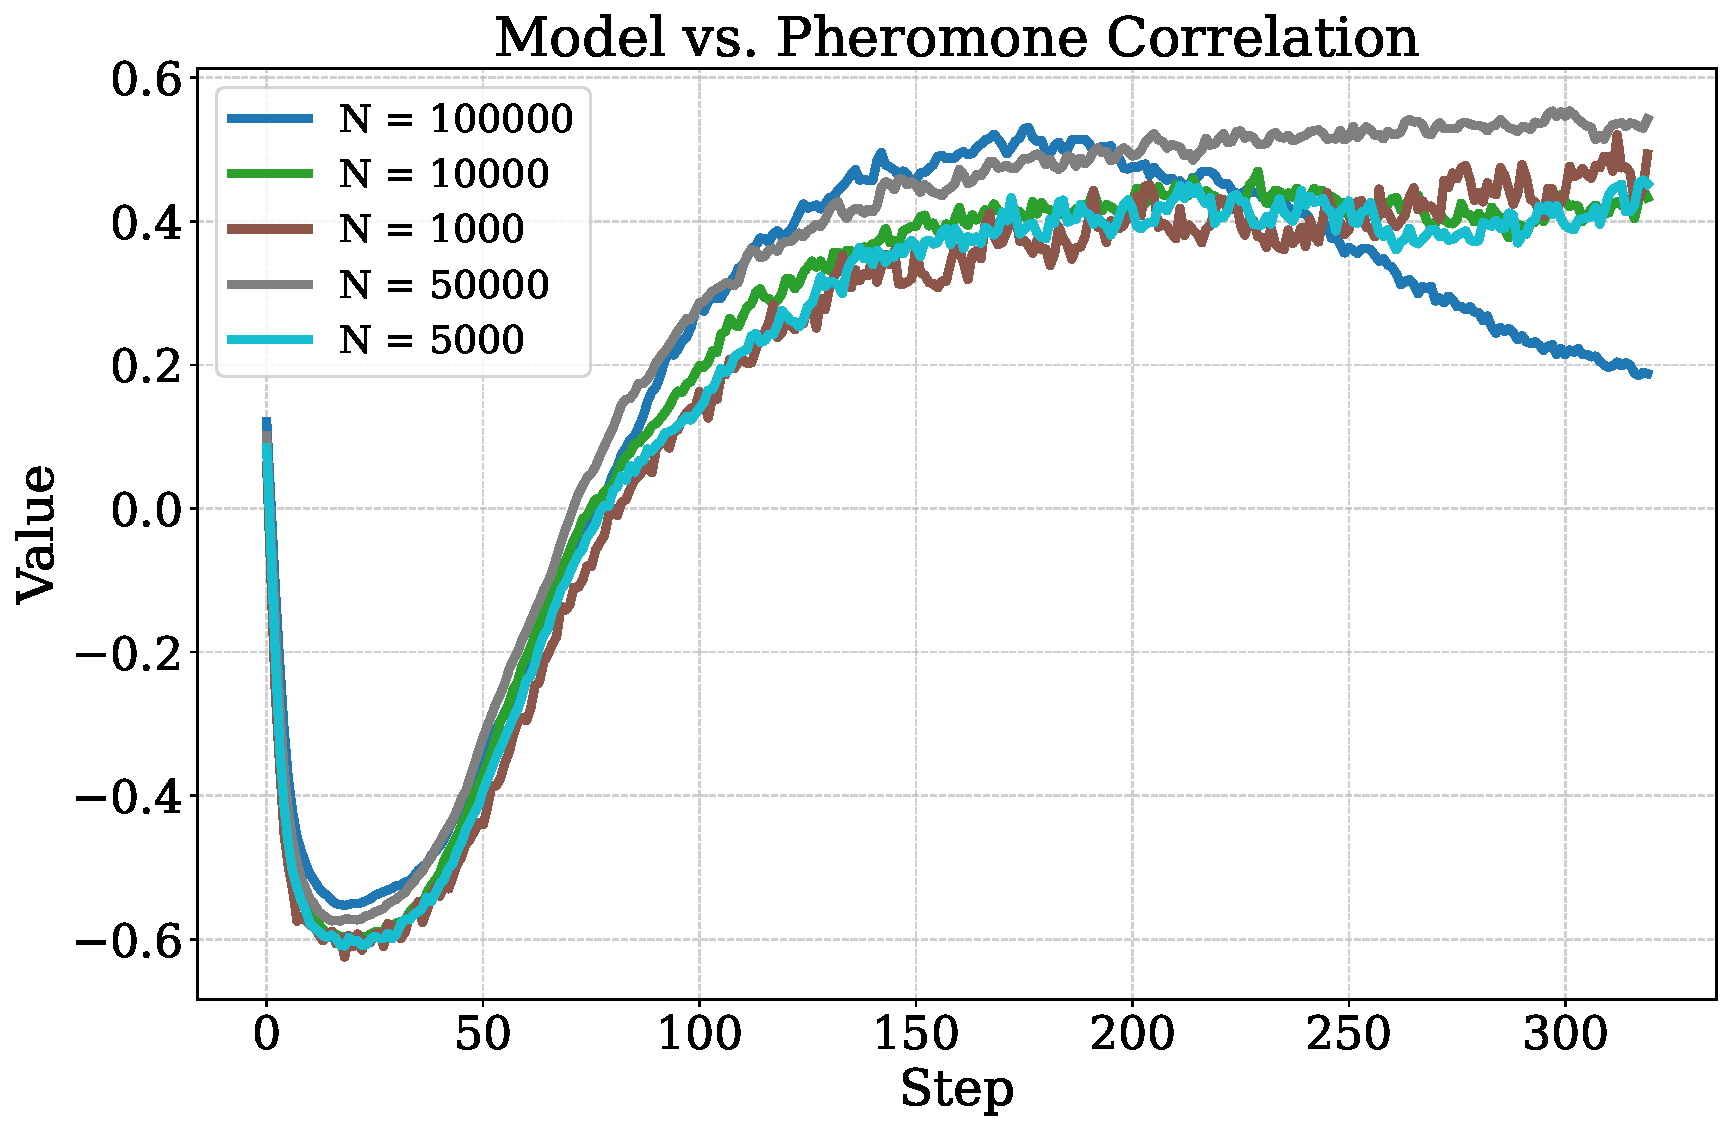
\includegraphics[width=\columnwidth]{figures/prior_eta_corr.pdf}
    \caption{Pearson correlation between neural guidance scores and pheromone concentration over training steps, for $N{=}1$K--$100$K.}
    \label{fig:guidance_eta_corr}
\end{figure}

\begin{figure}[t]
    \centering
    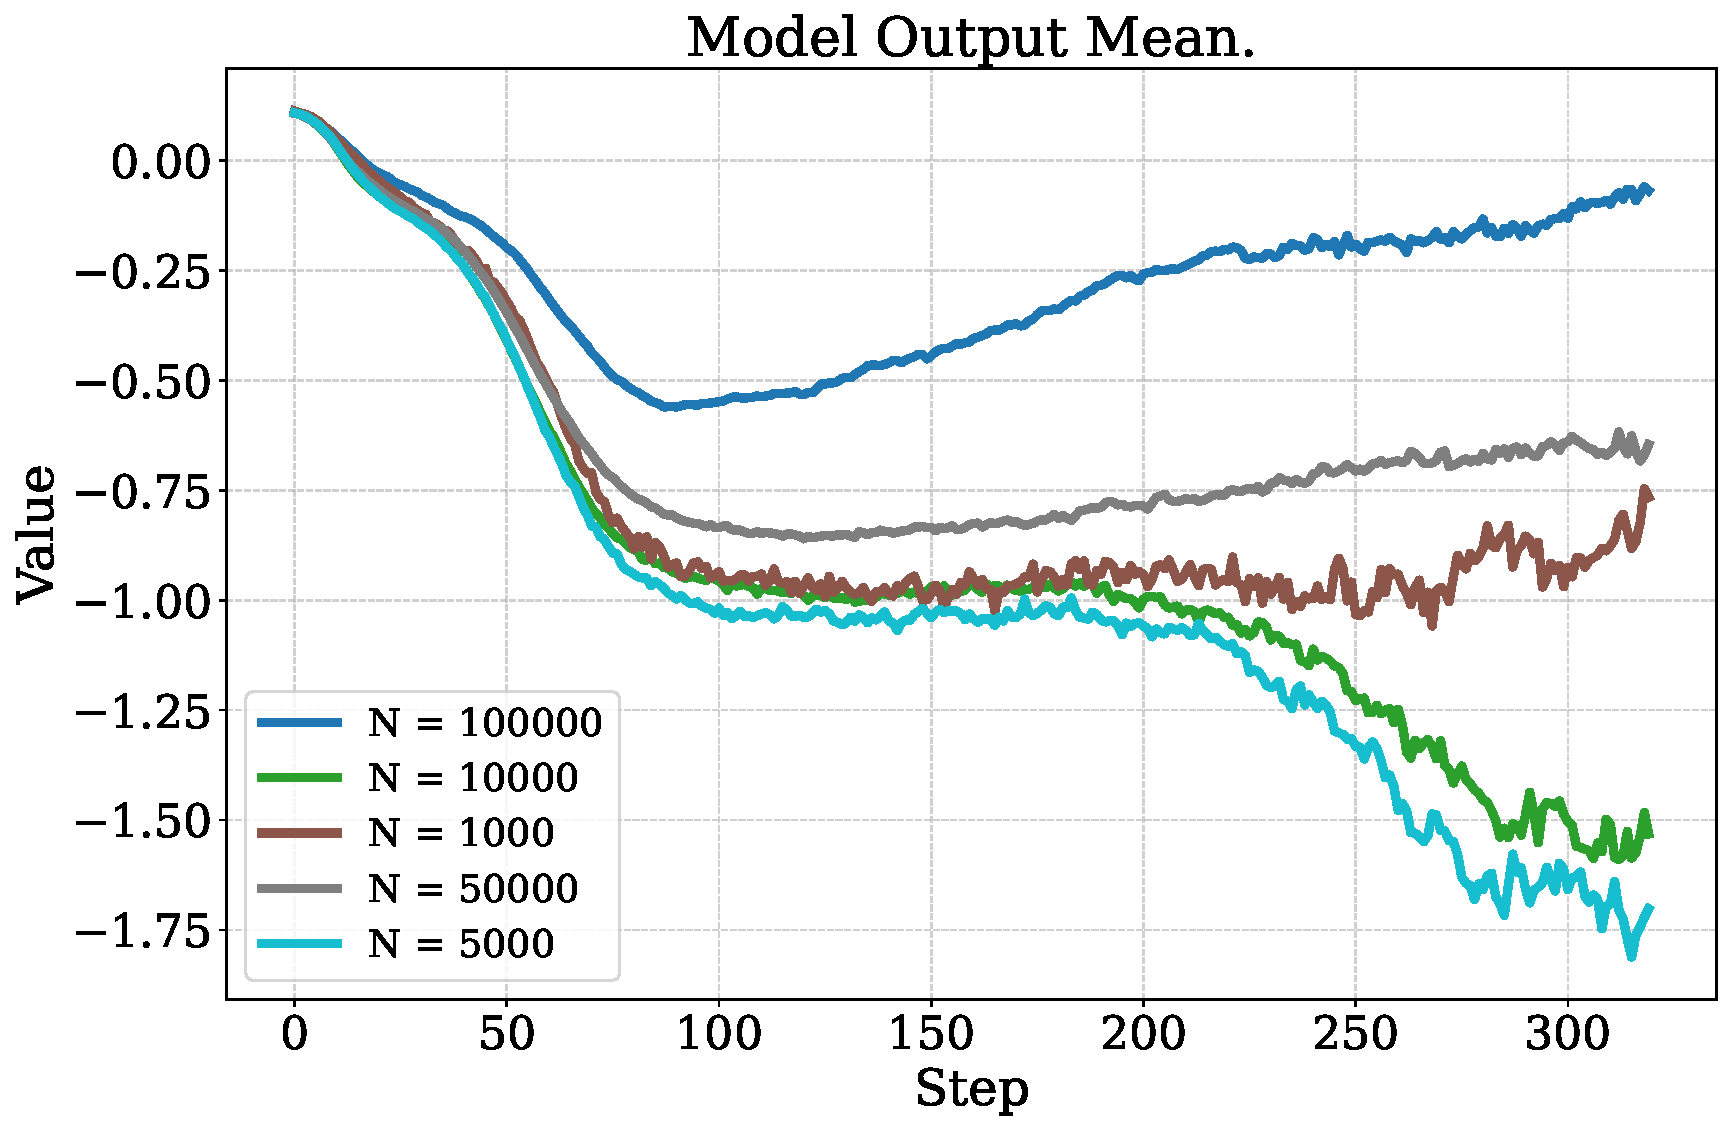
\includegraphics[width=\columnwidth]{figures/prior_mean.pdf}
    \caption{Mean neural guidance score over training steps, for $N{=}1$K--$100$K.}
    \label{fig:guidance_mean}
\end{figure}

\textbf{Cross-scale universality of the correlation trajectory.}
Despite an order-of-magnitude difference in problem size, the guidance--pheromone correlation follows a strikingly consistent trajectory across all scales (Figure~\ref{fig:guidance_eta_corr}): an initial sharp decrease in the early training phase, followed by a gradual recovery.
This pattern suggests a universal two-phase learning dynamic: the policy first learns to \emph{diverge} from the pheromone signal, establishing an independent, complementary guidance role, and subsequently learns to \emph{selectively re-align} with pheromone on edges where the two signals agree.
The near-identical evolution across scales provides further evidence that the state-aware representation generalizes across problem sizes, consistent with the cross-scale transfer results in the main paper.

\textbf{Scale-dependent variation in guidance magnitude.}
In contrast to the correlation trajectory, the mean guidance value (Figure~\ref{fig:guidance_mean}) exhibits modest scale-dependent differences.
Most notably, the $N{=}100$K and $N{=}5$K curves both start at lower mean values, but diverge during training: the $N{=}100$K mean rises back toward zero while the $N{=}5$K mean remains lower.
Nevertheless, a consistent finding across \emph{all} scales is that the mean guidance remains negative throughout training.
This indicates that, for TSP, the learned policy predominantly assumes a \emph{suppressive} role with respect to the pheromone field: down-weighting over-reinforced edges rather than amplifying under-explored ones.
This observation is consistent with the anti-stagnation behavior discussed in the main paper: since ACO's positive-feedback loop systematically over-concentrates pheromone, a complementary policy that applies net-negative corrections provides the most effective guidance strategy.

\textbf{CVRP: capacity constraints induce chaotic correlation dynamics.}
Figures~\ref{fig:guidance_eta_corr_cvrp} and~\ref{fig:guidance_mean_cvrp} replicate the above analysis for CVRP.
The guidance--pheromone correlation (Figure~\ref{fig:guidance_eta_corr_cvrp}) is markedly more volatile than the smooth, scale-invariant trajectory observed for TSP.
We attribute this to the heterogeneous capacity constraints that define CVRP: as problem size increases, the number of routes, their load distributions, and the feasibility landscape all change qualitatively, preventing the policy from settling into a single, universal correlation regime.
Unlike TSP, where the combinatorial structure is homogeneous across scales, CVRP's capacity dimension introduces a confounding factor that makes the guidance--pheromone relationship inherently scale-dependent.

\begin{figure}[t]
    \centering
    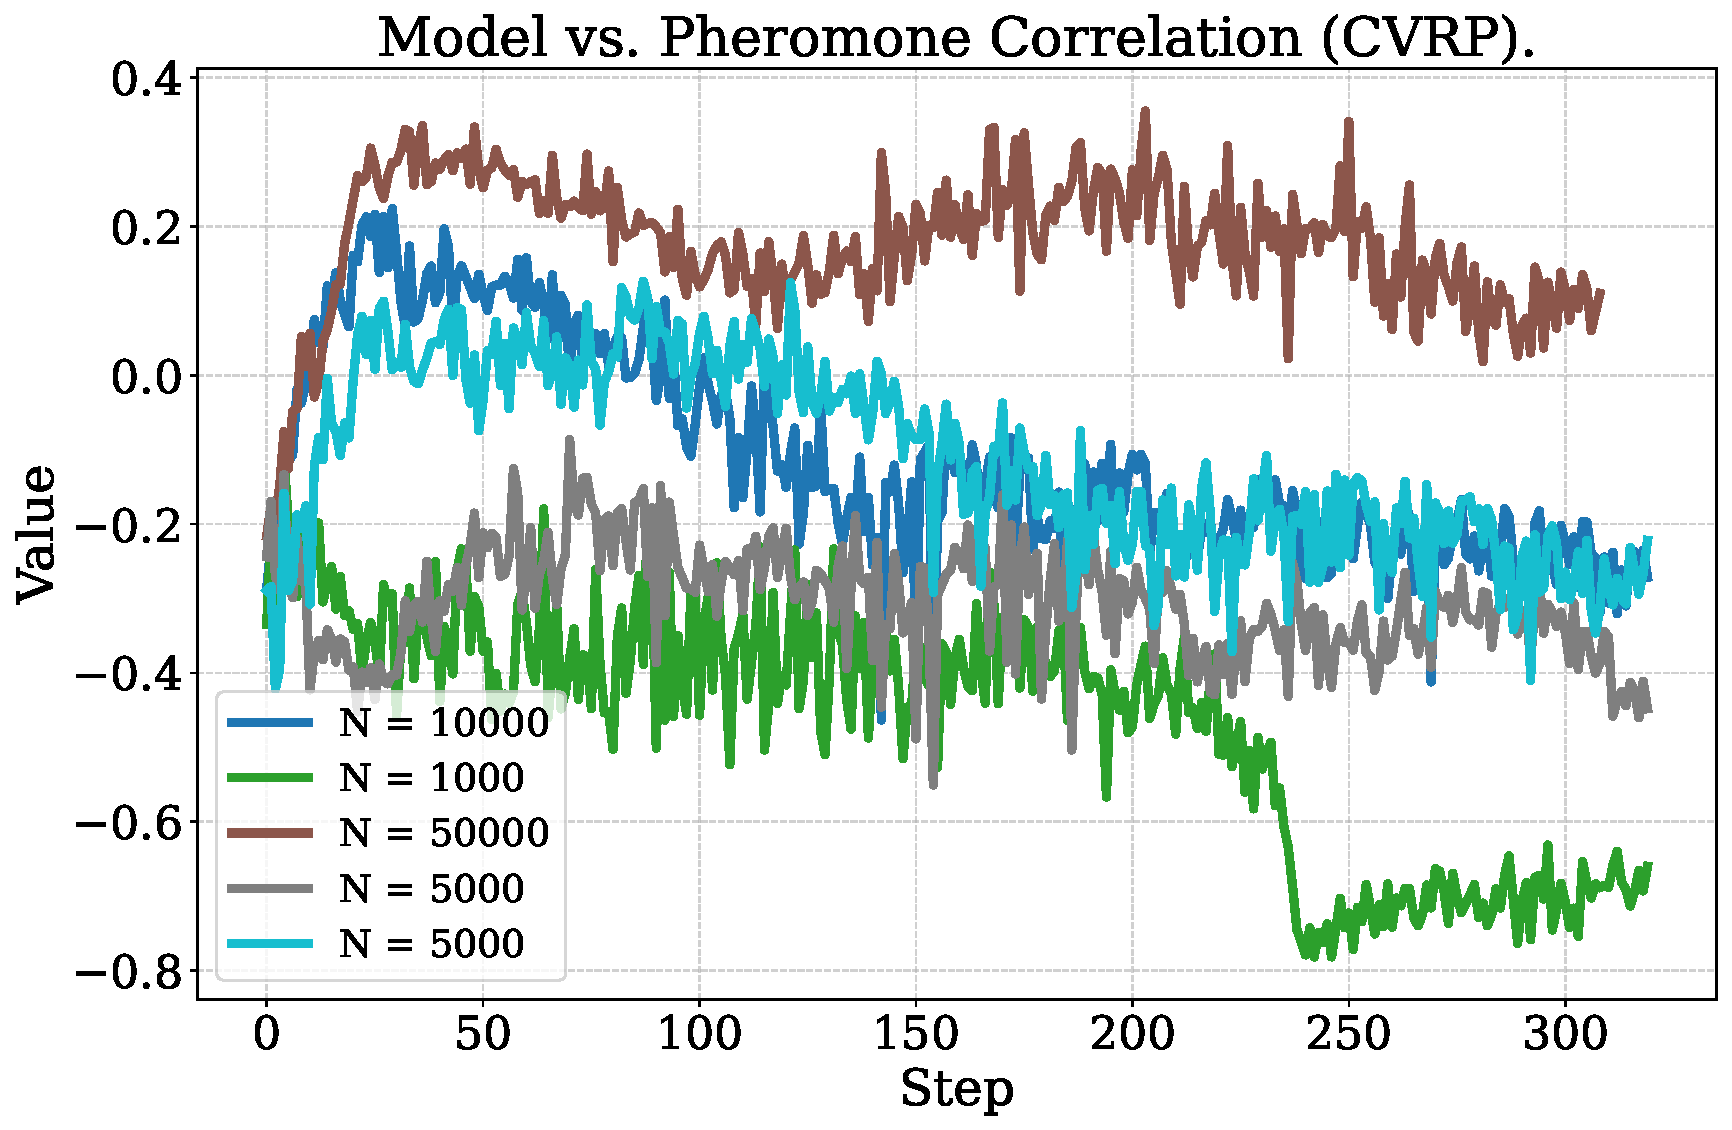
\includegraphics[width=\columnwidth]{figures/corr_cvrp.pdf}
    \caption{Pearson correlation between neural guidance scores and pheromone concentration over training steps for CVRP, $N{=}1$K--$50$K.}
    \label{fig:guidance_eta_corr_cvrp}
\end{figure}

\begin{figure}[t]
    \centering
    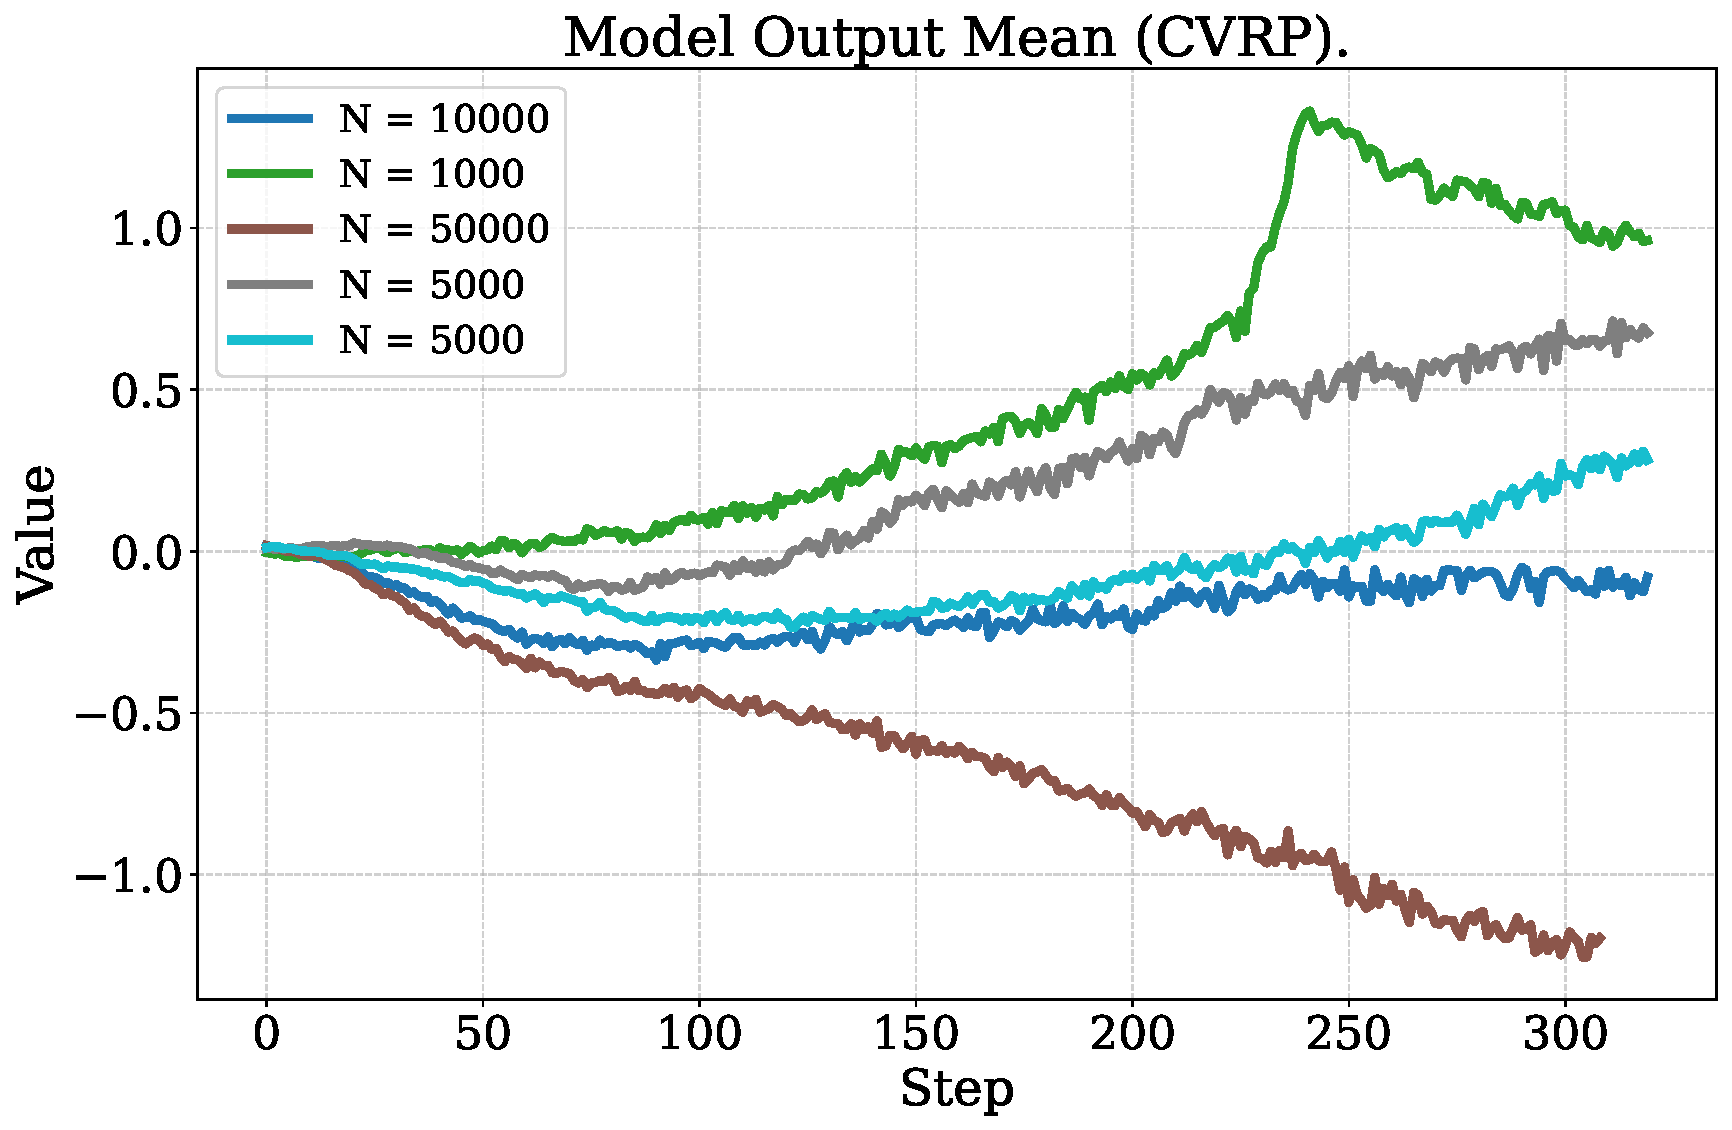
\includegraphics[width=\columnwidth]{figures/mean_cvrp.pdf}
    \caption{Mean neural guidance score over training steps for CVRP, $N{=}1$K--$50$K.}
    \label{fig:guidance_mean_cvrp}
\end{figure}


\begin{figure}[t]
    \centering
    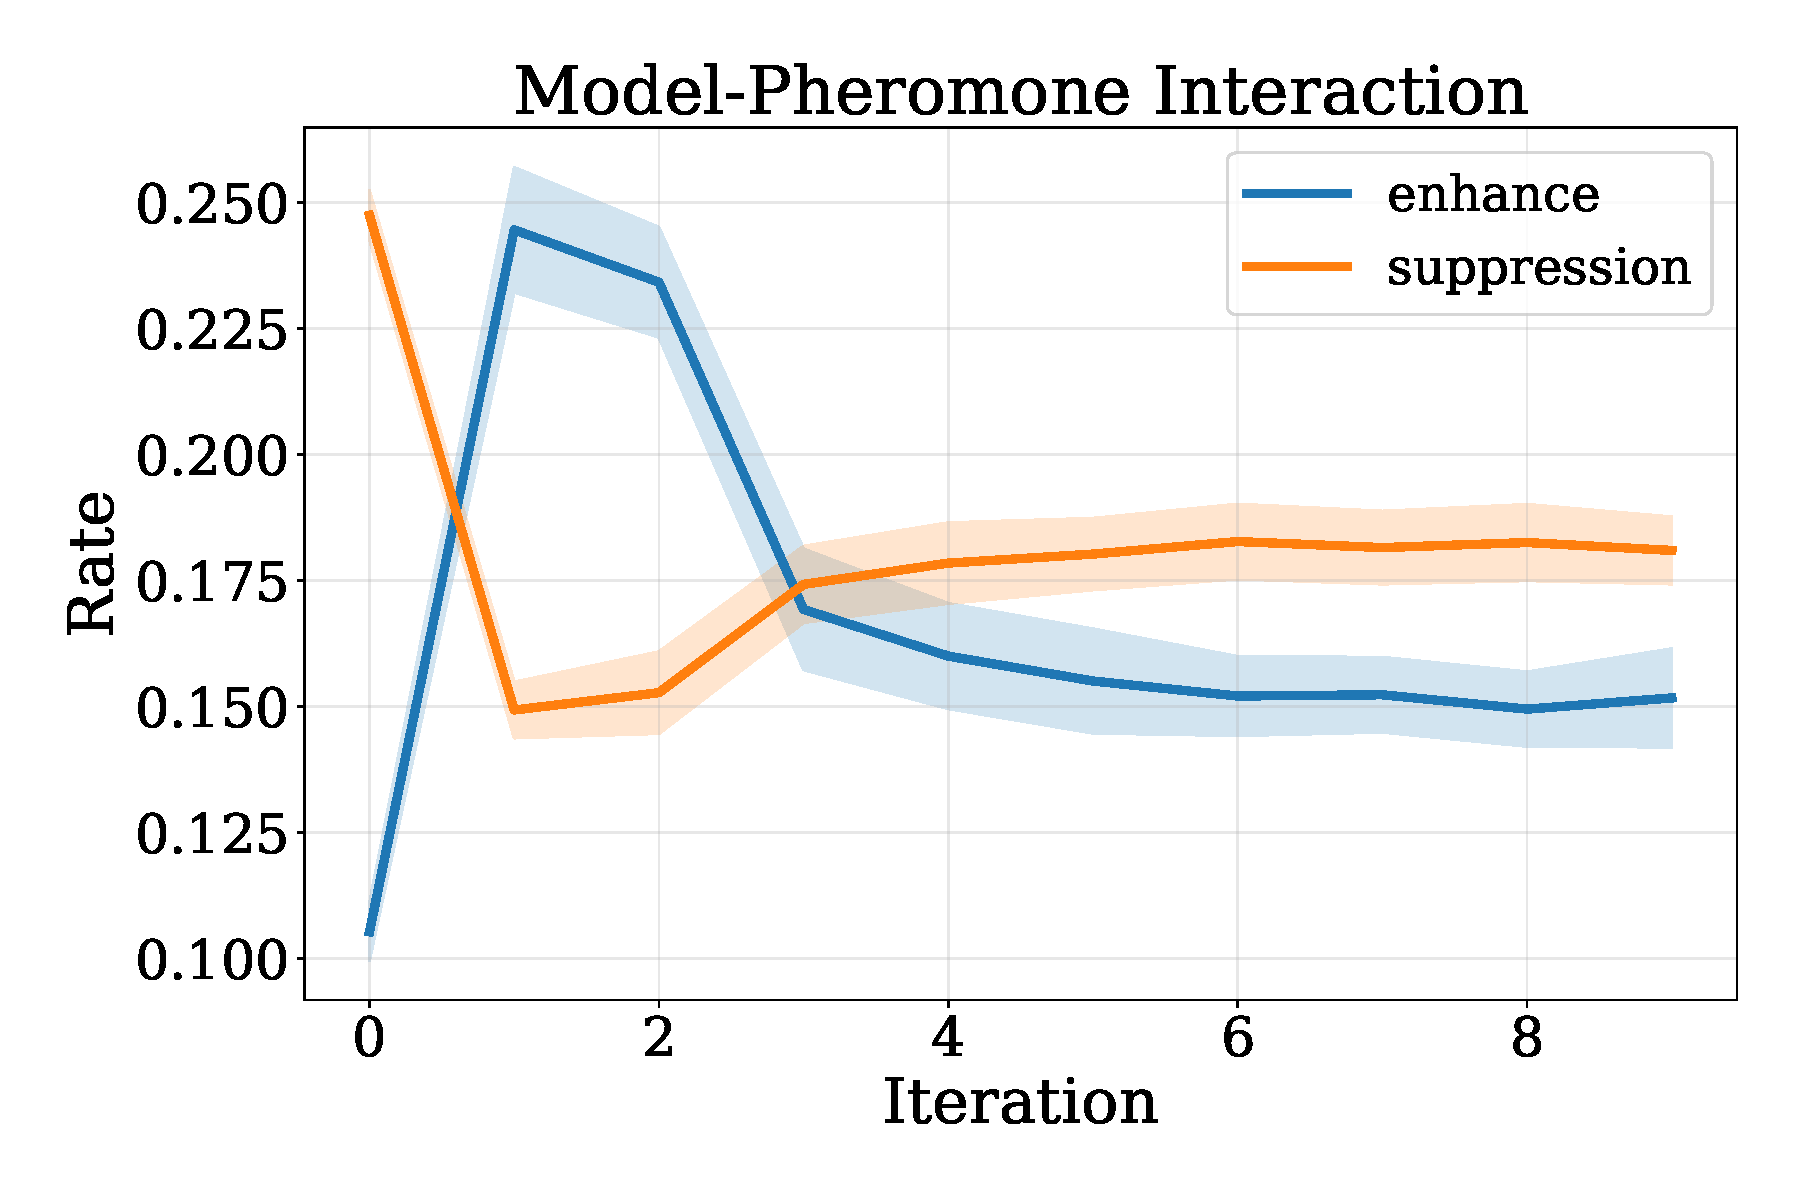
\includegraphics[width=\columnwidth]{figures/interaction.pdf}
    \caption{Guidance--pheromone interaction rates (enhancement vs.\ suppression) across outer steps $H{=}1$--$10$.}
    \label{fig:interaction}
\end{figure}


\begin{figure}[t]
    \centering
    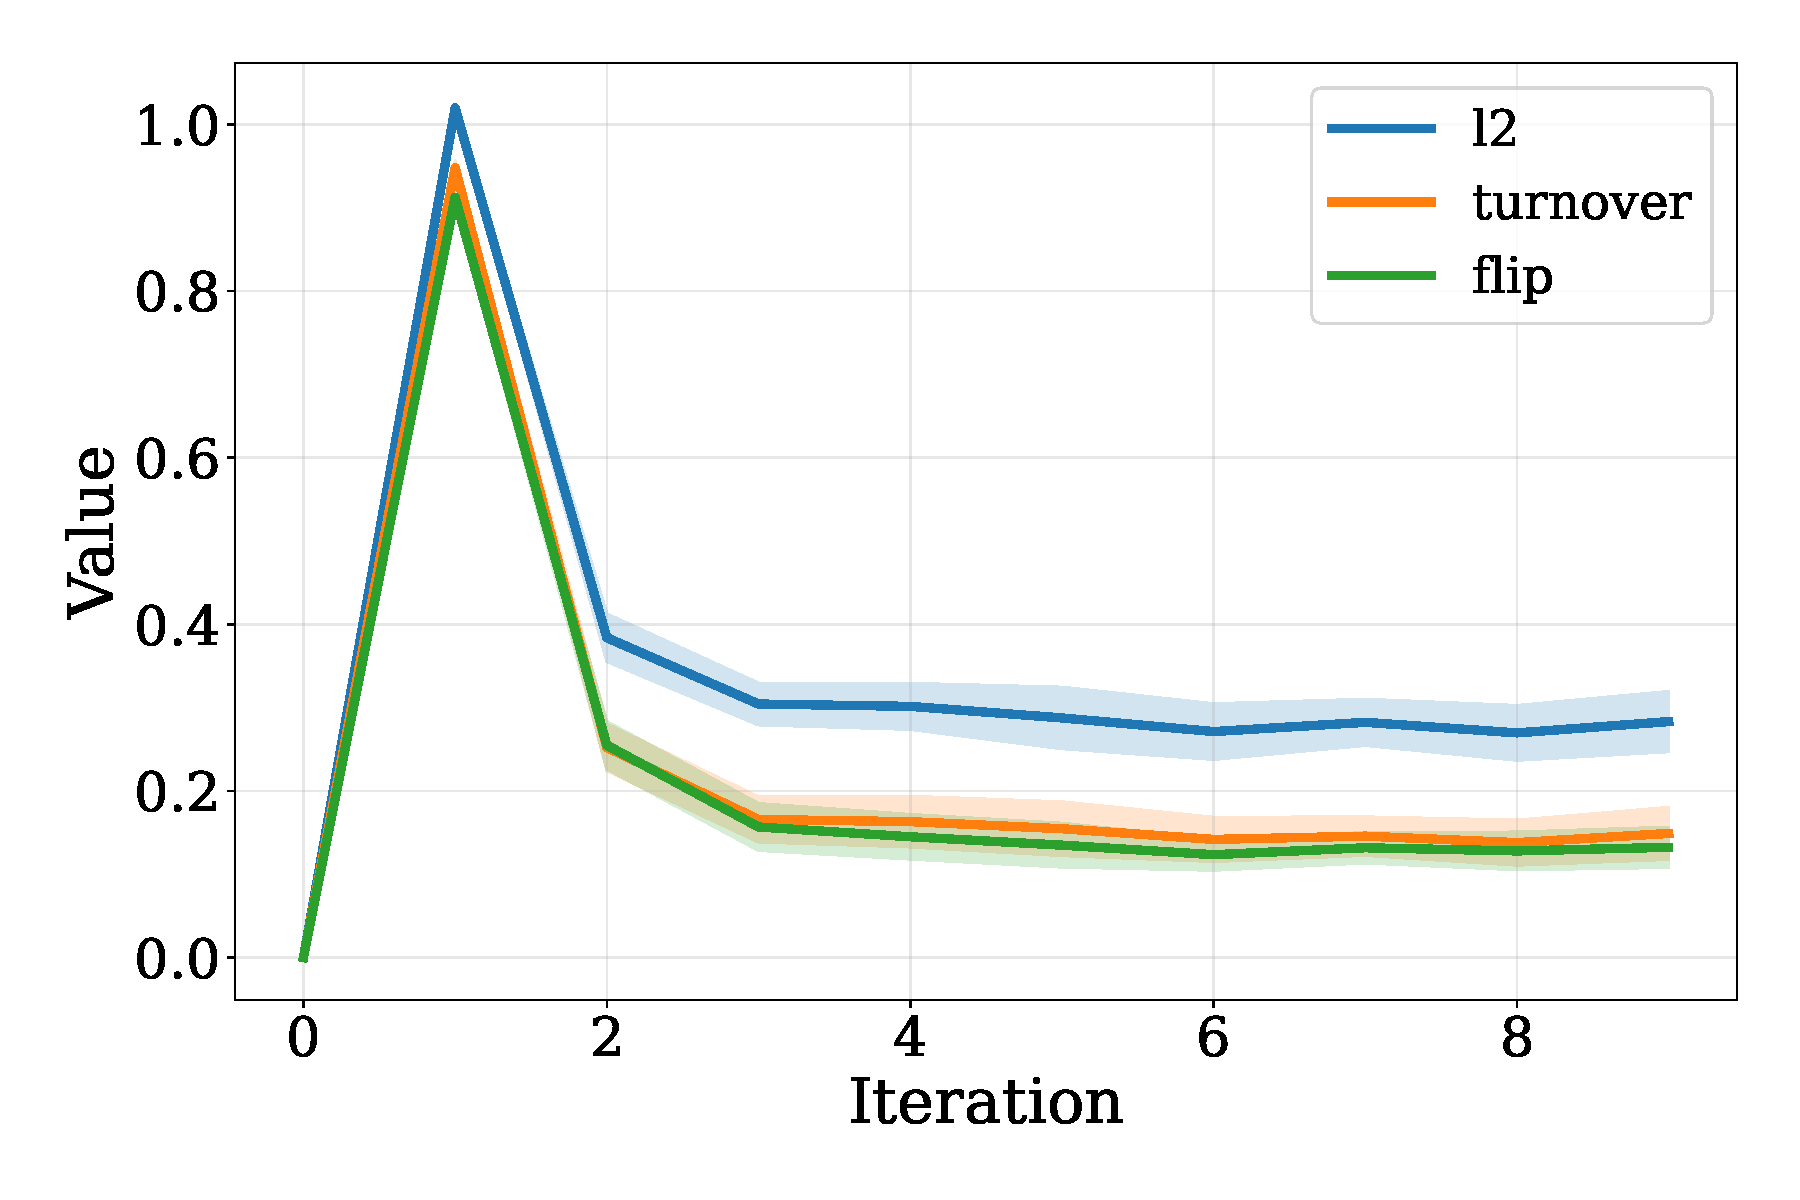
\includegraphics[width=\columnwidth]{figures/prior_changes.pdf}
    \caption{Guidance volatility metrics ($\ell_2$ drift, top-set turnover, argmax flip rate) across outer steps $H{=}1$--$10$.}
    \label{fig:prior_changes}
\end{figure}

\textbf{Guidance undergoes a rapid initial adaptation followed by steady-state refinement.}
Figure~\ref{fig:prior_changes} tracks three complementary measures of guidance change between consecutive outer steps: the relative $\ell_2$ drift, the top-set turnover (Jaccard distance among the top-5\% edges), and the argmax flip rate (fraction of nodes whose highest-guidance neighbor changes).
All three metrics spike to ${\sim}1.0$ at the first outer step ($H{=}1$), indicating that the policy substantially revises its guidance upon first observing pheromone feedback.
After this initial adjustment, all metrics stabilize at ${\sim}0.2$--$0.3$ and remain there for the subsequent nine outer steps, indicating that the policy settles into a regime of incremental, fine-grained updates conditioned on the gradually evolving pheromone landscape.

\begin{figure}[t]
    \centering
    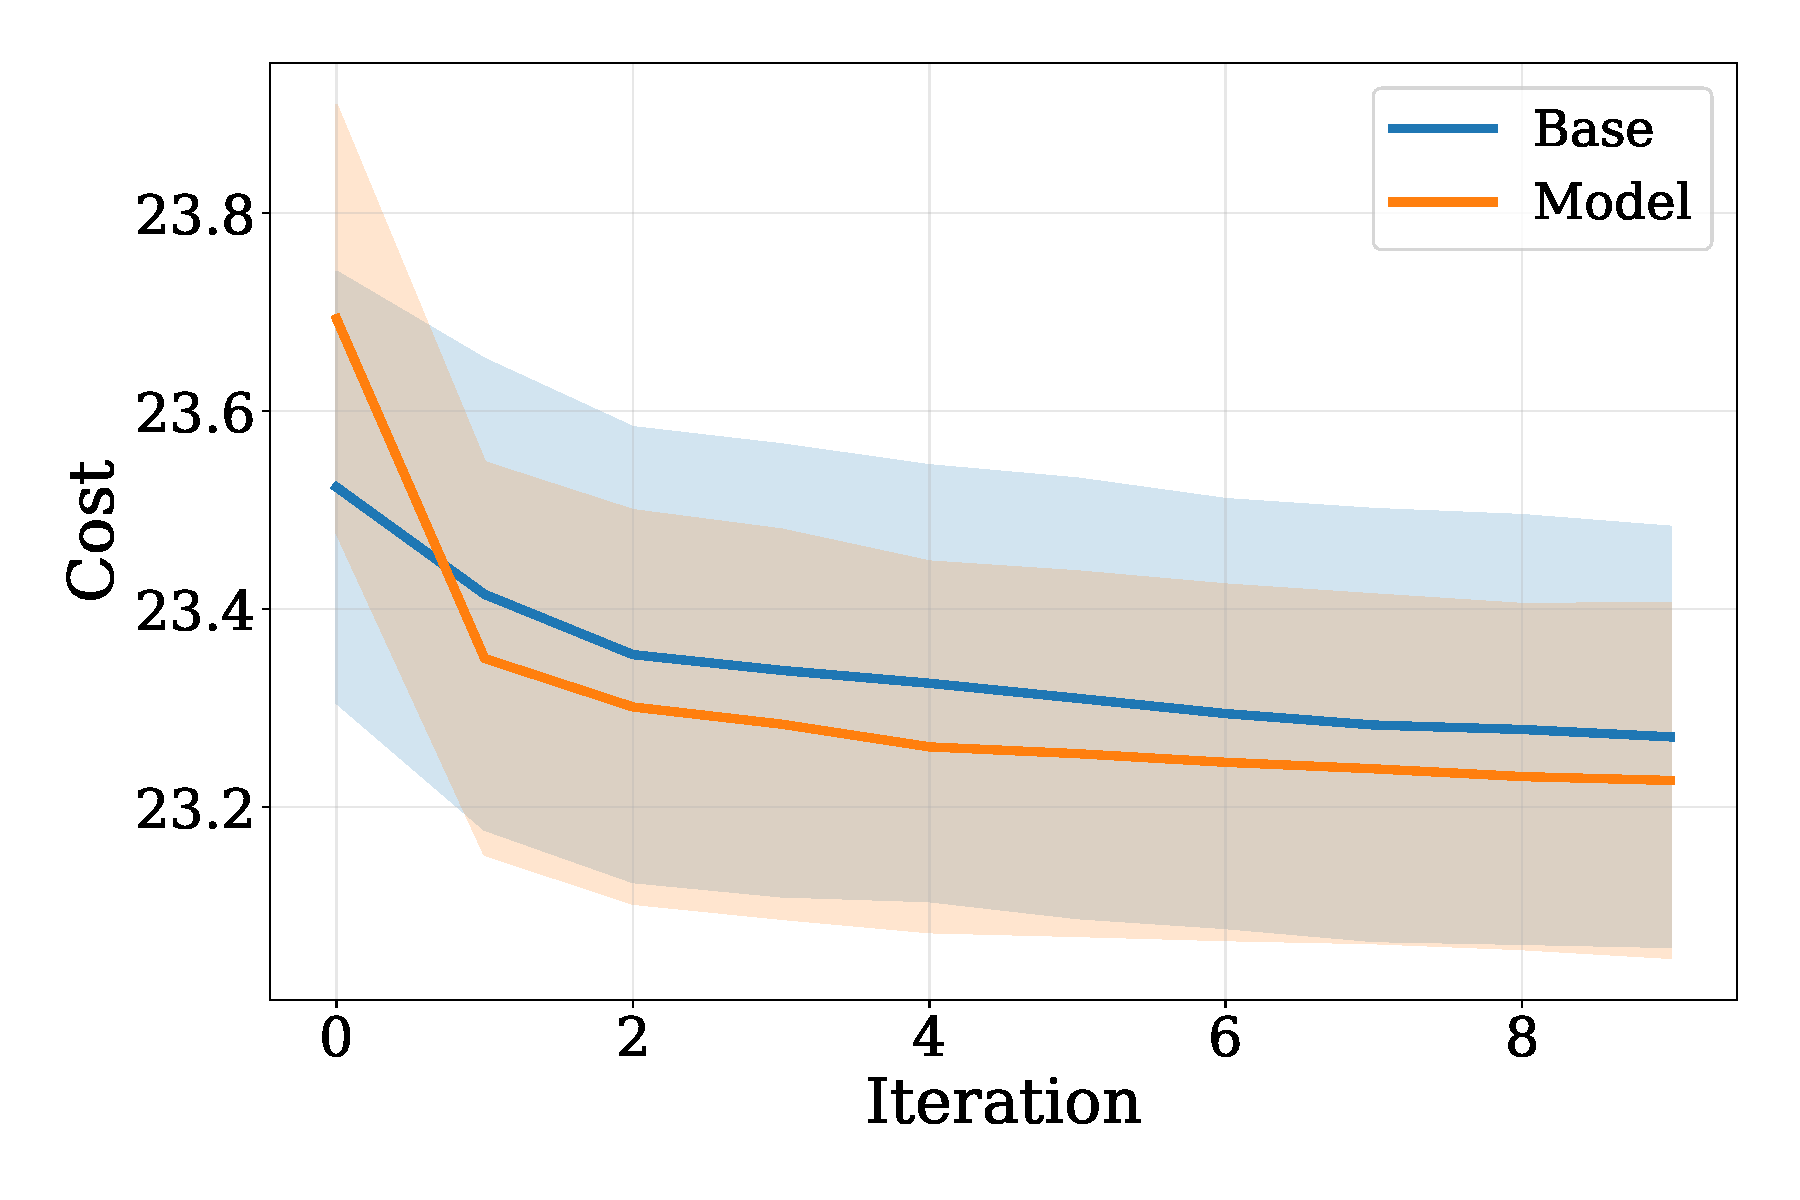
\includegraphics[width=\columnwidth]{figures/cost.pdf}
    \caption{Costs of DyNACO and ACO.}
    \label{fig:cost}
\end{figure}


\begin{figure}[t]
    \centering
    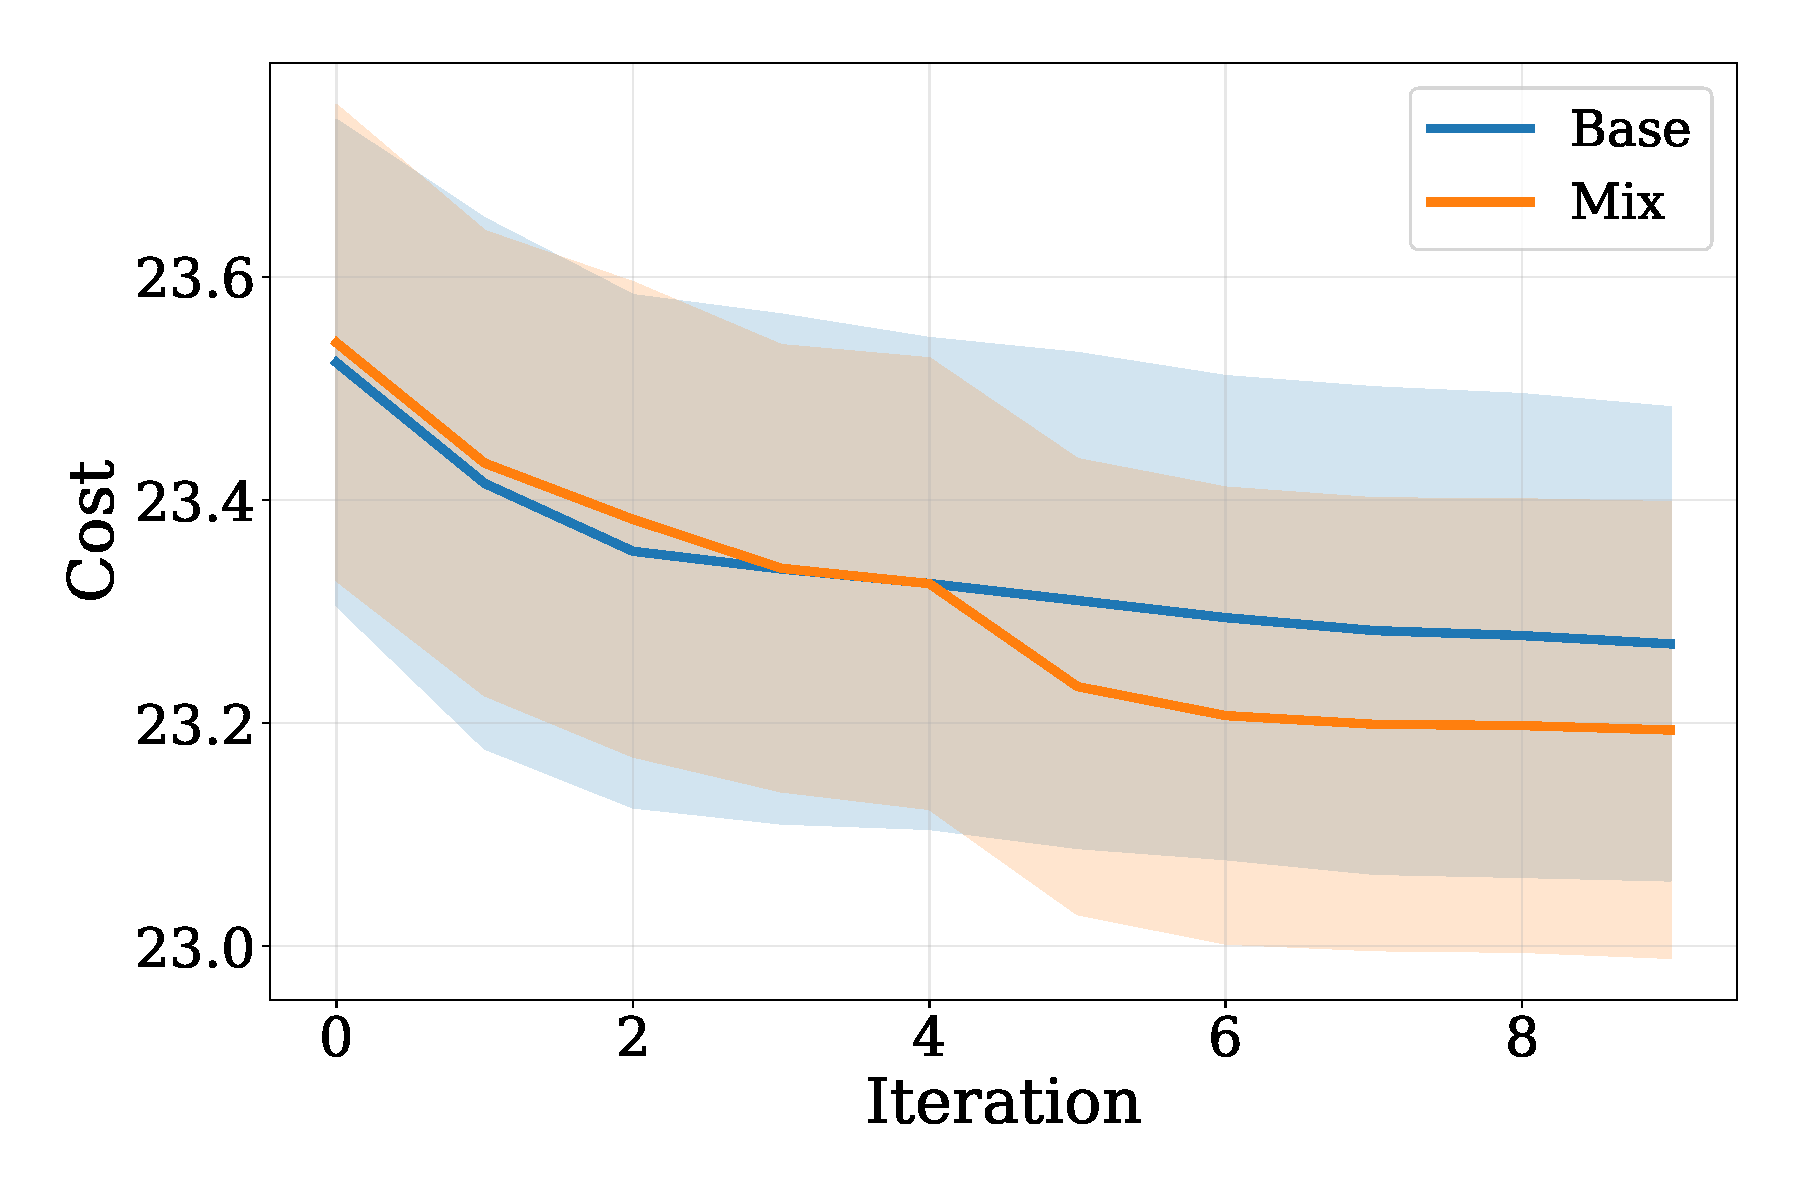
\includegraphics[width=\columnwidth]{figures/cost_mix.pdf}
    \caption{Costs of DyNACO and ACO (Phased Guidance).}
    \label{fig:cost-mix}
\end{figure}

\textbf{The policy transitions from enhancement to suppression over the search trajectory.}
Figure~\ref{fig:interaction} decomposes the guidance--pheromone interaction into two modes: \emph{enhancement} (edges ranked in the top-$k$ by both pheromone and guidance, indicating agreement) and \emph{suppression} (edges ranked in the top-$k$ by pheromone but bottom-$k$ by guidance, indicating active opposition).
At $H{=}1$, enhancement spikes to ${\sim}0.24$ while suppression drops to ${\sim}0.15$, reflecting a cooperative phase in which the policy reinforces early pheromone signals.
By $H{=}3$, the two curves cross: suppression overtakes enhancement and remains dominant through $H{=}10$, with suppression trending gradually upward and enhancement trending downward.
This crossover is an empirical transition learned by PPO as the marginal utility of guidance changes over the search trajectory, rather than an analytically derived switching point.
In early search, pheromone fields are near-uniform and carry limited information; the policy cooperates by amplifying the few edges that show early promise.
As pheromone concentrates and ACO's positive-feedback loop risks premature convergence, the policy shifts to a predominantly suppressive role, counteracting over-reinforced edges to maintain solution diversity.
This adaptive transition from cooperative to adversarial guidance is precisely the behavior that trajectory-aware training incentivizes and that static priors, which lack access to the evolving pheromone state, fundamentally cannot exhibit.

\textbf{CVRP: scale-dependent guidance polarity.}
The mean guidance trajectory (Figure~\ref{fig:guidance_mean_cvrp}) reveals a further contrast with TSP.
Whereas TSP scales share a common starting point before diverging modestly, CVRP scales separate early and evolve in opposing directions: the $N{=}1$K mean steadily increases toward $+1.0$, while the $N{=}50$K mean decreases toward $-1.0$.
This polarity reversal indicates that the optimal guidance strategy is qualitatively different across CVRP scales.
At small scales, capacity constraints are relatively loose and pheromone fields converge quickly; the policy learns to \emph{amplify} the existing pheromone signal, reinforcing promising routes.
At large scales, the combinatorial explosion of feasible route partitions makes pheromone concentration premature; the policy instead adopts the same suppressive, anti-stagnation role observed in TSP, counteracting over-reinforcement to maintain diversity.
Despite this divergence, each scale's trajectory is individually stable, suggesting that the policy consistently converges to a well-defined strategy conditioned on the problem characteristics encoded in the state representation.

% ======================================================================
% Appendix D: Additional Results
% ======================================================================
\section{Additional Results}
\label{app:results}

% ----------------------------------------------------------------------
\subsection{Inference Strategy Ablation}
\label{app:inference}

The model is always trained with constant guidance ($\gamma{=}1$) over the full trajectory, without annealing or phased scheduling.
At inference, two temporal strategies serve as problem- and scale-specific hyperparameters.
Table~\ref{tab:inference-config} summarizes the configuration used for each reported result.

\begin{table}[h]
\centering
\caption{Inference strategy configuration per problem and scale.}
\label{tab:inference-config}
\small
\begin{tabular}{lcc}
\toprule
Setting & Annealing & Phased Injection \\
\midrule
TSP-1K (all budgets)          & \checkmark & \checkmark \\
TSP-5K, 10K, 50K, 100K       & \checkmark &            \\
CVRP (all scales, $I{<}5000$) &            &            \\
CVRP (all scales, $I{\geq}5000$) &         & \checkmark \\
\bottomrule
\end{tabular}
\end{table}

\textbf{Guidance Annealing (TSP only).}
Annealing $\gamma \to 0$ linearly across inner iterations transitions from neural steering to pheromone exploitation:
\begin{equation}
\lim_{t \to T} P_t(j \mid i) \propto (\tau_{ij})^\alpha (\eta_{ij})^\beta.
\end{equation}
This strategy is effective for TSP, where pheromone dynamics on unconstrained tours converge reliably; once the colony has concentrated pheromone on promising edges, neural bias becomes redundant and may impede fine-grained pheromone exploitation.
For CVRP, however, capacity constraints fragment routes into many short vehicle tours whose structure depends on demand distributions.
Pheromone convergence is less uniform across these segments, and premature removal of neural guidance risks exploiting suboptimal route decompositions.
Accordingly, $\gamma{=}1$ is maintained throughout CVRP inference.

\textbf{Phased Injection.}
An injection threshold $\phi \in [0,1]$ controls when neural guidance activates.
For the first $\phi \cdot H$ outer steps, the solver operates with vanilla ACO only; at step $\lceil\phi \cdot H\rceil$, neural shaping logits are injected.
For TSP-1K, phased injection is applied at all iteration budgets because the small scale allows sufficient pheromone diversity to develop quickly.
For larger TSP scales, phased injection is not used: every outer step is valuable and delaying activation forfeits a significant fraction of the budget.
For CVRP, phased injection is applied only at longer iteration budgets ($I{\geq}5000$), where early pheromone fields are too uniform for the policy to provide meaningful direction; at shorter horizons, constant guidance is preferred.
Training on the full trajectory ($0 \to T$) with randomized warmup ensures the policy handles both high-entropy (exploratory) and low-entropy (converged) pheromone states at deployment.

\textbf{Training vs.\ inference asymmetry.}
While annealing $\gamma \to 0$ improves inference performance, it is counterproductive during training: the gradient scales as $\nabla_\theta \log P_t(j \mid i) \propto \gamma_t \cdot \nabla_\theta z_\theta(i,j)$, so as $\gamma_t \to 0$ the gradient signal vanishes.
Training therefore always maintains constant $\gamma{=}1$, preserving gradient magnitude across the full trajectory and ensuring the policy learns from all search phases.
The inference strategies above are strictly post-hoc enhancements applied to this single trained model.

\begin{table}[h]
\centering
\caption{Inference strategy ablation. Gap (\%) to LKH-3. All models trained with constant $\gamma{=}1$; strategies applied post-hoc.}
\label{tab:ablation-inference}
\small
\begin{tabularx}{\columnwidth}{lYYYY}
\toprule
Inference Strategy & TSP5K & TSP10K & CVRP5K & CVRP10K \\
\midrule
Constant ($\gamma{=}1$)            & 1.38 & 1.73 & \textbf{6.58} & 11.16 \\
Phased injection           & \textbf{1.20} & 1.68 & 7.07 & \textbf{10.86} \\
Guidance annealing         & 1.23 & \textbf{1.59} & 6.84 & 11.17 \\
Phased + Annealing         & 1.23 & 1.60 & 7.35 & 11.02 \\
\bottomrule
\end{tabularx}
\end{table}

Table~\ref{tab:ablation-inference} ablates all four strategy combinations on TSP and CVRP.
For TSP, annealing and phased injection is consistently beneficial.
For CVRP, phased injection at long horizons provides modest gains, while annealing degrades performance.

\textbf{Training with inference strategies degrades performance.}
A natural question is whether incorporating these strategies \emph{during training} would produce a better-matched policy.
Table~\ref{tab:train-strategy} evaluates this on TSP-5K ($I_{1000}$) by training separate models under each of the four strategy combinations and evaluating every model with all four inference strategies.
In every case, the model trained with constant $\gamma{=}1$ over the full trajectory yields the best result, regardless of which inference strategy is applied.
Training with annealing causes the policy gradient to vanish in later iterations ($\nabla_\theta \propto \gamma_t \to 0$), preventing the policy from learning effective late-stage guidance.
Training with phased injection withholds the policy from early search phases, reducing the diversity of pheromone states observed during optimization.
These results confirm that the training--inference asymmetry is not merely a convenience but a necessity: the gradient signal must be preserved across all search phases during training, and inference strategies should be applied strictly post-hoc.

\begin{table}[h]
\centering
\caption{Training regime vs.\ inference strategy on TSP-5K ($I_{1000}$). Gap (\%) to LKH-3. Each row trains with a different strategy; each column applies a different inference strategy. Best per-column in bold.}
\label{tab:train-strategy}
\small
\begin{tabular}{lcccc}
\toprule
& \multicolumn{4}{c}{Inference Strategy} \\
\cmidrule(lr){2-5}
Training Regime & Constant & Anneal & Phased & Phased+Anneal \\
\midrule
Constant $\gamma{=}1$ (ours)               & 1.39 & 1.24 & 1.21 & 1.28 \\
Anneal $\gamma{\to}0$                       & 1.31 & 1.35 & 1.23 & 1.23 \\
Phased ($\phi{=}0.5$)                       & 1.37 & 1.26 & 1.24 & 1.25 \\
\bottomrule
\end{tabular}
\end{table}

% ----------------------------------------------------------------------
\subsection{TSPLIB Real-World Instances}
\label{app:tsplib}

Table~\ref{tab:tsplib} reports per-instance results on 33 TSPLIB instances (1K--86K nodes) using the TSP-1K model with $I_{10000}$.
We compare three configurations: unguided ACO, DyNACO with guidance annealing only, and DyNACO$^{\dagger}$ with phased injection.

\begin{table}[h]
\centering
\caption{TSPLIB per-instance results (TSP-1K model, $I_{10000}$). Gap (\%) relative to known optima.}
\label{tab:tsplib}
\small
\renewcommand{\arraystretch}{0.85}
\begin{tabularx}{\columnwidth}{lYYYY}
\toprule
Instance & $n$ & ACO & DyNACO & DyNACO$^{\dagger}$ \\
\midrule
\multicolumn{5}{l}{\textit{In-distribution scale ($n \leq 2{,}500$)}} \\
\midrule
\texttt{dsj1000}  & 1,000 & 0.74 & \textbf{0.40} & 0.69 \\
\texttt{pr1002}   & 1,002 & 0.75 & 0.68 & \textbf{0.47} \\
\texttt{u1060}    & 1,060 & 0.60 & 0.63 & \textbf{0.47} \\
\texttt{vm1084}   & 1,084 & 0.20 & 0.54 & \textbf{0.14} \\
\texttt{pcb1173}  & 1,173 & 0.85 & \textbf{0.81} & 1.09 \\
\texttt{d1291}    & 1,291 & 1.04 & 1.14 & \textbf{0.89} \\
\texttt{rl1304}   & 1,304 & 1.68 & \textbf{0.96} & 1.06 \\
\texttt{rl1323}   & 1,323 & 0.22 & 1.22 & \textbf{0.19} \\
\texttt{nrw1379}  & 1,379 & 1.17 & \textbf{0.81} & \textbf{0.81} \\
\texttt{fl1400}   & 1,400 & 1.65 & 2.11 & \textbf{1.01} \\
\texttt{u1432}    & 1,432 & 1.03 & 0.73 & \textbf{0.46} \\
\texttt{fl1577}   & 1,577 & 0.34 & \textbf{0.23} & \textbf{0.23} \\
\texttt{d1655}    & 1,655 & \textbf{1.14} & 1.24 & 1.22 \\
\texttt{vm1748}   & 1,748 & 0.61 & \textbf{0.26} & 0.39 \\
\texttt{u1817}    & 1,817 & 1.72 & 1.77 & \textbf{1.53} \\
\texttt{rl1889}   & 1,889 & 0.31 & \textbf{0.05} & 0.65 \\
\texttt{d2103}    & 2,103 & 0.55 & 0.53 & \textbf{0.45} \\
\texttt{u2152}    & 2,152 & 2.03 & 2.63 & \textbf{1.77} \\
\texttt{u2319}    & 2,319 & 1.25 & 1.27 & \textbf{1.12} \\
\texttt{pr2392}   & 2,392 & 1.41 & 1.05 & \textbf{0.60} \\
\midrule
\multicolumn{5}{l}{\textit{Out-of-distribution scale ($n > 2{,}500$)}} \\
\midrule
\texttt{pcb3038}  & 3,038 & 1.42 & \textbf{0.64} & 0.69 \\
\texttt{fl3795}   & 3,795 & 3.15 & 1.87 & \textbf{0.94} \\
\texttt{fnl4461}  & 4,461 & 2.24 & 1.37 & \textbf{1.27} \\
\texttt{rl5915}   & 5,915 & 1.07 & 1.37 & \textbf{0.96} \\
\texttt{rl5934}   & 5,934 & \textbf{0.85} & 1.02 & 0.94 \\
\texttt{pla7397}  & 7,397 & 1.29 & 1.03 & \textbf{0.83} \\
\texttt{rl11849}  & 11,849 & 1.38 & 1.10 & \textbf{0.67} \\
\texttt{usa13509} & 13,509 & 1.19 & 1.13 & \textbf{0.92} \\
\texttt{brd14051} & 14,051 & 2.22 & 1.30 & \textbf{1.16} \\
\texttt{d15112}   & 15,112 & 1.98 & 1.19 & \textbf{1.18} \\
\texttt{d18512}   & 18,512 & 2.37 & 1.37 & \textbf{1.33} \\
\texttt{pla33810} & 33,810 & 1.84 & 1.71 & \textbf{1.59} \\
\texttt{pla85900} & 85,900 & 2.25 & 1.78 & \textbf{1.65} \\
\midrule
\textbf{Avg.~(all)} & -- & 1.29 & 1.09 & \textbf{0.89} \\
\textbf{Avg.~($n{\leq}2.5$K)} & -- & 0.96 & 0.95 & \textbf{0.76} \\
\textbf{Avg.~($n{>}2.5$K)} & -- & 1.79 & 1.28 & \textbf{1.09} \\
\bottomrule
\end{tabularx}
\vspace{2pt}

\raggedright\footnotesize{DyNACO = model-only with annealing; DyNACO$^{\dagger}$ = phased injection with best of anneal/no-anneal per instance. All gaps in \%. DyNACO$^{\dagger}$ outperforms ACO on 29/33 instances.}
\end{table}

% ----------------------------------------------------------------------
\subsection{CVRPlib Real-World Instances}
\label{app:cvrplib}

Table~\ref{tab:cvrplib} reports per-instance results on 14 CVRPlib instances (1K--30K customers) using the CVRP-1K model with $I_{10000}$.

\begin{table}[h]
\centering
\caption{CVRPlib per-instance results (CVRP-1K model, $I_{10000}$). Gap (\%) relative to BKS.}
\label{tab:cvrplib}
\small
\renewcommand{\arraystretch}{0.85}
\begin{tabularx}{\columnwidth}{lYYY}
\toprule
Instance & $n$ & ACO & DyNACO$^{\dagger}$ \\
\midrule
\multicolumn{4}{l}{\textit{In-distribution scale ($n \leq 2{,}500$)}} \\
\midrule
\texttt{Li\_30}        & 1,040  & 2.67 & \textbf{0.03} \\
\texttt{Li\_31}        & 1,120  & 2.66 & \textbf{2.38} \\
\texttt{Li\_32}        & 1,200  & 2.04 & \textbf{1.79} \\
\texttt{X-n1001-k43}  & 1,000  & 2.88 & \textbf{2.53} \\
\midrule
\multicolumn{4}{l}{\textit{Out-of-distribution scale ($n > 2{,}500$)}} \\
\midrule
\texttt{Leuven1}      & 3,000  & 2.17 & \textbf{1.75} \\
\texttt{Leuven2}      & 4,000  & 7.25 & \textbf{5.85} \\
\texttt{Antwerp1}     & 6,000  & 2.67 & \textbf{2.28} \\
\texttt{Antwerp2}     & 7,000  & 6.16 & \textbf{5.70} \\
\texttt{Ghent1}       & 10,000 & 2.32 & \textbf{2.26} \\
\texttt{Ghent2}       & 11,000 & 7.51 & \textbf{6.96} \\
\texttt{Brussels1}    & 15,000 & 3.29 & \textbf{2.98} \\
\texttt{Brussels2}    & 16,000 & 8.23 & \textbf{7.72} \\
\texttt{Flanders1}    & 20,000 & 2.16 & \textbf{1.93} \\
\texttt{Flanders2}    & 30,000 & 7.56 & \textbf{7.05} \\
\midrule
\textbf{Avg.~(all)}          & -- & 4.25 & \textbf{3.66} \\
\textbf{Avg.~($n{\leq}2.5$K)} & -- & 2.56 & \textbf{1.68} \\
\textbf{Avg.~($n{>}2.5$K)}   & -- & 4.93 & \textbf{4.45} \\
\bottomrule
\end{tabularx}
\vspace{2pt}

\raggedright\footnotesize{DyNACO$^{\dagger}$ = phased injection, no annealing. All gaps in \%. DyNACO$^{\dagger}$ outperforms ACO on 14/14 instances.}
\end{table}

% ----------------------------------------------------------------------
\subsection{Extended Ablation Tables}

\subsubsection{Environment Stabilization}

Table~\ref{tab:ablation-mmas-app} examines pheromone bound strategies.
Standard \MMAS{} couples bounds to solution cost, creating non-stationary dynamics.
Our stabilized variant ($\tau_{\max}{=}1$, $\tau_{\min}{=}1/K$) yields scale-invariant state representations and reduced training variance.

\begin{table}[h]
\centering
\caption{Environment stabilization. We report results without inference strategies.}
\label{tab:ablation-mmas-app}
\small
\renewcommand{\arraystretch}{0.85}
\begin{tabularx}{\columnwidth}{lYYY}
\toprule
Bound Strategy & Obj. & Gap (\%)\\
\midrule
ACO (Standard \MMAS{}) & 51.8318 & 1.68  \\
ACO (Stabilized) & 52.0747 & 2.16 \\
DyNACO (Standard \MMAS{}) & 51.7022 & 1.43 \\
DyNACO (Stabilized) & 51.6795 & 1.38 \\
\bottomrule
\end{tabularx}
\end{table}

\begin{table*}[t]
\centering
\caption{Sensitivity to outer guidance updates $H$ and inner ACO steps $S$.}
\label{tab:hs-sensitivity-app}
\small
\renewcommand{\arraystretch}{0.85}
\begin{tabularx}{\textwidth}{llYYYYYYYY}
\toprule
$H$ & $S$ & TSP-1K Obj. & Time & TSP-5K & Time & CVRP-1K & Time & CVRP-5K & Time \\
\midrule
5 & 200 & 23.22 & 0.32 & 51.59 & 0.75 & 36.62 & 1.34 & \textbf{96.16} & 3.07 \\
10 & 100 & 23.23 & \textbf{0.32} & 51.63 & \textbf{0.76} & \textbf{36.28} & \textbf{1.27} & 96.81 & \textbf{2.73} \\
20 & 50 & \textbf{23.21} & 0.42 & \textbf{51.56} & 0.87 & 36.49 & 1.33 & 97.17 & 2.82 \\
\bottomrule
\end{tabularx}
\end{table*}

\subsubsection{Memory Scaling}

Table~\ref{tab:memory-scaling} reports peak GPU memory usage for representative constructive and neural-ACO baselines.
Methods based on dense attention or dense heatmaps scale quadratically in the number of nodes and become infeasible at larger scales.
\DyNACO{} instead operates on a fixed-size sparse candidate graph and uses perturbation-based sampling, so memory scales approximately linearly with $n$ for fixed $K$.

\begin{table}[h]
\centering
\caption{Peak GPU memory usage (GB) on TSP instances. OOM: out of memory.}
\label{tab:memory-scaling}
\small
\renewcommand{\arraystretch}{0.85}
\begin{tabularx}{\columnwidth}{lYYYYY}
\toprule
Method & 1K & 5K & 10K & 50K & 100K \\
\midrule
POMO & 0.10 & 2.54 & 10.11 & OOM & OOM \\
SIGD & 0.04 & 0.95 & 3.76 & OOM & OOM \\
LEHD & 0.10 & 2.27 & 9.01 & OOM & OOM \\
DeepACO & 0.14 & 2.11 & 8.31 & OOM & OOM \\
\DyNACO{} & \textbf{0.08} & \textbf{0.18} & \textbf{0.35} & 1.57 & 3.11 \\
\bottomrule
\end{tabularx}
\end{table}

\subsubsection{Hyperparameter Sensitivity}

Table~\ref{tab:k-sensitivity-app} and Table~\ref{tab:m-sensitivity-app} evaluate the candidate-graph size $K$ and perturbation length $M$.
Larger $K$ improves quality with a near-linear runtime trade-off.
The best $M$ is problem-dependent: more perturbation steps are not automatically better, because excessive changes can disrupt the incumbent basin and increase refinement cost.

\begin{table}[h]
\centering
\caption{Sensitivity to candidate-graph size $K$.}
\label{tab:k-sensitivity-app}
\small
\renewcommand{\arraystretch}{0.85}
\begin{tabularx}{\columnwidth}{lYYYY}
\toprule
$K$ & TSP-5K & Time & CVRP-5K & Time \\
\midrule
32 & 51.63 & \textbf{0.76} & 96.81 & \textbf{2.73} \\
48 & 51.49 & 0.98 & 95.83 & 3.51 \\
64 & \textbf{51.47} & 1.17 & \textbf{95.08} & 4.42 \\
\bottomrule
\end{tabularx}
\end{table}

\begin{table}[h]
\centering
\caption{Sensitivity to perturbation length $M$.}
\label{tab:m-sensitivity-app}
\small
\renewcommand{\arraystretch}{0.85}
\begin{tabularx}{\columnwidth}{lYYYY}
\toprule
$M$ & TSP-5K & Time & CVRP-5K & Time \\
\midrule
8 & \textbf{51.62} & \textbf{0.73} & 97.13 & \textbf{2.37} \\
12 & 51.63 & 0.76 & 96.81 & 2.73 \\
16 & 51.77 & 0.82 & \textbf{96.48} & 3.24 \\
\bottomrule
\end{tabularx}
\end{table}

Table~\ref{tab:hs-sensitivity-app} varies the outer guidance updates $H$ and inner ACO steps $S$ while keeping the total iteration budget fixed.
\DyNACO{} remains robust across these temporal granularities, supporting the fixed-duration semi-MDP abstraction used in the main method.

\subsubsection{Capacity-Dependent Guidance in CVRP}

The polarity of learned guidance in CVRP is driven by route capacity rather than only by the number of feasible solutions.
Table~\ref{tab:capacity-guidance-app} shows that as capacity increases, the guidance mean rises monotonically while the pheromone correlation changes sign, matching the scale-dependent behavior observed in CVRP guidance trajectories.

\begin{table}[h]
\centering
\caption{Capacity-dependent guidance statistics on CVRP.}
\label{tab:capacity-guidance-app}
\small
\renewcommand{\arraystretch}{0.85}
\begin{tabularx}{\columnwidth}{lYYYY}
\toprule
Capacity & Obj. & Route & Guidance Mean & Pheromone Corr. \\
\midrule
100 & 70.87 & 50.44 & 0.15 & 0.72 \\
200 & 43.71 & 25.56 & 0.67 & -0.22 \\
250 & 37.37 & 20.62 & 0.96 & -0.18 \\
\bottomrule
\end{tabularx}
\end{table}

\subsubsection{Parameter and Feature Overhead}

\DyNACO{} adds dynamic state features to a compact GNN policy.
Using the architecture of Joshi et al.~\cite{deepaco}, increasing the edge-feature input from 1 to 6 adds only 160 parameters, from 67,201 to 67,361.
The peak GPU-memory overhead of these additional features remains small even at 100K nodes, as shown in Table~\ref{tab:feature-memory-app}.

\begin{table}[h]
\centering
\caption{Peak GPU memory (GB) for static and dynamic policy inputs.}
\label{tab:feature-memory-app}
\small
\renewcommand{\arraystretch}{0.85}
\begin{tabularx}{\columnwidth}{llYY}
\toprule
Problem & Scale & Static (GB) & Dynamic (GB) \\
\midrule
TSP & 10K & 0.286 & 0.293 \\
TSP & 100K & 2.524 & 2.584 \\
CVRP & 10K & 0.286 & 0.292 \\
CVRP & 100K & 2.513 & 2.573 \\
\bottomrule
\end{tabularx}
\end{table}

% ======================================================================
% Appendix E: Extended Background and Baseline Analysis
% ======================================================================
\section{Extended Background and Baseline Analysis}
\label{app:related}

\subsection{The Training--Inference Misalignment in Static Guidance}
\label{app:static-bottleneck}

Neural-guided ACO methods (DeepACO~\cite{deepaco}, GFACS~\cite{gfacs}, GTG-ACO~\cite{gtgaco}) train a model to emit edge heuristics from instance geometry.
All optimize a \emph{single-step} objective: $\min_\theta \mathbb{E}_{\pi \sim p_\theta(\cdot \mid G)} [ C(\pi) ]$, where a single batch of ants samples tours guided only by the neural heuristic, without pheromone, without an incumbent, and without iterative feedback.
At inference, however, this static heatmap is integrated into a full ACO loop where pheromone fields evolve over hundreds of iterations, creating a clear misalignment between training conditions and deployment conditions.

Under this paradigm, any model producing edge scores serves the same role.
HeatACO~\cite{heataco} confirms this empirically: generic heatmap models (AttGCN, DIMES, DIFUSCO) match or exceed ACO-specific architectures in the same pipeline, suggesting that the bottleneck lies in the static integration rather than the model architecture.

Because guidance is computed only once, the fixed heatmap may conflict with the pheromone landscape as it evolves during search, potentially degrading performance in later iterations.
\DyNACO{} addresses this limitation through dynamic neural guidance: the state-aware representation exposes the evolving pheromone field and incumbent to the policy, while trajectory-aware training over $H{=}10$ outer steps optimizes the policy to provide effective guidance throughout the search.

% ----------------------------------------------------------------------
\subsection{Credit Assignment under Local Search: Neural Local Search vs.\ Scope-Restricted Refinement}
\label{app:nls-analysis}

Training on post-local-search rewards is difficult because discrete LS operators can wash out the policy-gradient credit signal connecting sampled actions to final rewards.
DeepACO addresses this via Neural Local Search (NLS), which injects neural priors into the LS acceptance criterion.

\textbf{Computational cost.}
NLS requires $O(N \cdot K)$ neural forward passes \emph{inside} the inner loop, for every ant, at every LS iteration.
For $m{=}100$ ants with $10{\times}$ neural refinement passes, this creates a $1000{\times}$ multiplier on neural inference cost.
At $N{=}500$ this cost is manageable; at $N{=}10{,}000$ it becomes the computational bottleneck, and at $N{=}100{,}000$ it is prohibitive.

Furthermore, NLS creates a dependency on dense refinement applied to \emph{every} ant, yet scalable heuristics typically apply LS \emph{sparsely} (e.g., every $k$ iterations) and \emph{elitely} (e.g., only to top solutions).

\textbf{SRR's alternative.}
Scope-Restricted Refinement, the scalability enabler of dynamic neural guidance, preserves policy-reward attribution by limiting the \emph{scope} of the update, not the \emph{nature} of the operator.
Because the incumbent is already locally optimal, perturbations create only localized regions of sub-optimality.
SRR repairs these regions to convergence using fast C++ heuristics (2-opt, or-opt), without any neural overhead.
This preserves the causal link between neural decisions and rewards while allowing use of highly optimized LS backends.
This distinction is also what makes SRR a scalability mechanism rather than merely a different local-search schedule: full LS can improve an individual tour but may erase policy attribution, whereas truncated LS preserves more attribution at the cost of leaving tours under-refined.

% ----------------------------------------------------------------------
\subsection{Scalability of Constructive Baselines}
\label{app:constructive-limits}

End-to-end constructive policies~\cite{attentionmodel,pomo,bq,lehd, invit, sigd} are typically trained on small-scale instances ($N{=}50$ or $100$) and rely on quadratic attention complexity $O(N^2)$ in the encoder.
When applied to large-scale instances ($N{\geq}1{,}000$), these models suffer from out-of-distribution degradation, as the learned representations do not transfer across scales, compounded by memory exhaustion from the $O(N^2)$ encoder.
The ``OOM'' entries in the main results table reflect this inherent limitation.
Prior neural-ACO methods have the same dense bottleneck in a different form: they materialize heatmap or pheromone-prior matrices in $\mathbb{R}^{N\times N}$ and are typically evaluated only up to $N{\leq}1000$, so scaling the full ACO loop induces an $O(N^2 m T)$ memory/computation burden across ants and iterations.

\textbf{Decomposition attempts.}
Recent methods address this through divide-and-conquer (GLOP~\cite{glop}, H-TSP~\cite{htsp}) or hierarchical construction (SIL~\cite{sil}, LEHD~\cite{lehd}).
However, decomposition methods depend on global context embeddings that degrade at extreme scales, and hierarchical methods incur prohibitive runtimes (SIL PRC$_{1000}$: 42h at TSP-100K).

\textbf{Sparse-graph scaling.}
\DyNACO{} operates on fixed-size $K$-NN neighborhoods ($K{=}32$), so the GNN processes each neighborhood identically regardless of $N$.
GPU memory is proportional to $n \cdot K$, not $n^2$, and per-ant sampling cost is $O(M \cdot K)$, independent of problem size.
At TSP-100K, DyNACO I$_{10000}$ completes in 46 minutes; SIL PRC$_{1000}$ requires 42 hours.

% ----------------------------------------------------------------------
\subsection{Ant Colony Optimization and Adaptive Control}
\label{app:aco-background}

Perturbation-based ACO~\cite{partialACO, P-ACO, faco} bounds differences between newly constructed solutions and the incumbent, yielding focused search with tighter LS coupling.
A natural question is whether a learned policy can further improve this family by conditioning on the evolving solver state.

Adapting ACO parameters during search has a long history.
\emph{Adaptive} or \emph{self-adaptive} ACO variants dynamically adjust evaporation rates, pheromone bounds, or exploration parameters based on search progress~\cite{adaptant,adaptant2}.
These methods typically rely on hand-crafted rules (e.g., restart upon stagnation, increase $\rho$ when diversity drops).
By contrast, dynamic neural guidance is \emph{learned} from data: the state-aware representation conditions on richer features (per-edge pheromone distribution, incumbent topology) rather than scalar metrics, and trajectory-aware training optimizes the policy to exploit these features effectively across the full search trajectory.
Prior work has explored pheromone information as features for learning.
RLACO~\cite{rlant} uses RL to tune global ACO parameters based on convergence metrics.
To our knowledge, no prior neural ACO method conditions on per-edge pheromone statistics to produce \emph{edge-level} guidance during search; existing approaches either tune global parameters or use pheromone summaries for meta-level decisions.
In contrast, \DyNACO{}'s dynamic neural guidance operates at a finer level of granularity: rather than selecting operators or tuning scalars, the state-aware policy directly shapes per-edge transition probabilities within a fixed operator (perturbative ACO sampling), providing search-phase-dependent guidance at the cost of requiring differentiable integration with the sampling process.

\bibliographystyle{plain}
\bibliography{references}

\end{document}

